\documentclass[review]{elsarticle}

\usepackage{lineno}
\usepackage{xspace}
\modulolinenumbers[5]

\journal{Annals of Nuclear Energy}

%% `Elsevier LaTeX' style
\bibliographystyle{elsarticle-num}
%%%%%%%%%%%%%%%%%%%%%%%

%%%% packages and definitions (optional)
\usepackage{placeins}
\usepackage{booktabs} % nice rules (thick lines) for tables
\usepackage{microtype} % improves typography for PDF
\usepackage{hhline}
\usepackage{amsmath}

%\usepackage[demo]{graphicx}
%\usepackage{caption}
%\usepackage{subcaption}

\usepackage{booktabs}
\usepackage{threeparttable, tablefootnote}

\usepackage{tabularx}
\newcolumntype{b}{>{\hsize=1.0\hsize}X}
\newcolumntype{s}{>{\hsize=.5\hsize}X}
\newcolumntype{m}{>{\hsize=.75\hsize}X}
\newcolumntype{x}{>{\hsize=.25\hsize}X}

\graphicspath{{figures/}}

% tikz %
\usepackage{tikz}
\usetikzlibrary{positioning, arrows, decorations, shapes}

\usetikzlibrary{shapes.geometric,arrows}
\tikzstyle{process} = [rectangle, rounded corners, minimum width=3cm, minimum height=1cm,text centered, draw=black, fill=blue!30]
\tikzstyle{object} = [ellipse, rounded corners, minimum width=3cm, minimum height=1cm,text centered, draw=black, fill=green!30]
\tikzstyle{arrow} = [thick,->,>=stealth]

% hyperref %
\usepackage[hidelinks]{hyperref}
% after hyperref %
\usepackage{cleveref}
\usepackage{datatool}
\usepackage[acronym,toc]{glossaries}
%\newacronym{<++>}{<++>}{<++>}
\newacronym[longplural={metric tons of heavy metal}]{MTHM}{MTHM}{metric ton of heavy metal}
\newacronym{ABM}{ABM}{agent-based modeling}
\newacronym{ACDIS}{ACDIS}{Program in Arms Control \& Domestic and International Security}
\newacronym{AHTR}{AHTR}{Advanced High Temperature Reactor}
\newacronym{ANDRA}{ANDRA}{Agence Nationale pour la gestion des D\'echets RAdioactifs, the French National Agency for Radioactive Waste Management}
\newacronym{ANL}{ANL}{Argonne National Laboratory}
\newacronym{ANS}{ANS}{American Nuclear Society}
\newacronym{API}{API}{application programming interface}
\newacronym{ARE}{ARE}{Aircraft Reactor Experiment}
\newacronym{ARFC}{ARFC}{Advanced Reactors and Fuel Cycles}
\newacronym{ASME}{ASME}{American Society of Mechanical Engineers}
\newacronym{ATWS}{ATWS}{Anticipated Transient Without Scram}
\newacronym{BDBE}{BDBE}{Beyond Design Basis Event}
\newacronym{BIDS}{BIDS}{Berkeley Institute for Data Science}
\newacronym{CAFCA}{CAFCA}{ Code for Advanced Fuel Cycles Assessment }
\newacronym{CDTN}{CDTN}{Centro de Desenvolvimento da Tecnologia Nuclear}
\newacronym{CEA}{CEA}{Commissariat \`a l'\'Energie Atomique et aux \'Energies Alternatives}
\newacronym{CFD}{CFD}{Computational Fluid Dynamics}
\newacronym{CI}{CI}{continuous integration}
\newacronym{CNEN}{CNEN}{Comiss\~{a}o Nacional de Energia Nuclear}
\newacronym{CNERG}{CNERG}{Computational Nuclear Engineering Research Group}
\newacronym{COSI}{COSI}{Commelini-Sicard}
\newacronym{COTS}{COTS}{commercial, off-the-shelf}
\newacronym{CSNF}{CSNF}{commercial spent nuclear fuel}
\newacronym{CTAH}{CTAHs}{Coiled Tube Air Heaters}
\newacronym{CUBIT}{CUBIT}{CUBIT Geometry and Mesh Generation Toolkit}
\newacronym{CURIE}{CURIE}{Centralized Used Fuel Resource for Information Exchange}
\newacronym{DAG}{DAG}{directed acyclic graph}
\newacronym{DANESS}{DANESS}{Dynamic Analysis of Nuclear Energy System Strategies}
\newacronym{DBE}{DBE}{Design Basis Event}
\newacronym{DESAE}{DESAE}{Dynamic Analysis of Nuclear Energy Systems Strategies}
\newacronym{DHS}{DHS}{Department of Homeland Security}
\newacronym{DOE}{DOE}{Department of Energy}
\newacronym{DRACS}{DRACS}{Direct Reactor Auxiliary Cooling System}
\newacronym{DRE}{DRE}{dynamic resource exchange}
\newacronym{DSNF}{DSNF}{DOE spent nuclear fuel}
\newacronym{DYMOND}{DYMOND}{Dynamic Model of Nuclear Development }
\newacronym{EBS}{EBS}{Engineered Barrier System}
\newacronym{EDF}{EDF}{Électricité de France}
\newacronym{EDZ}{EDZ}{Excavation Disturbed Zone}
\newacronym{EIA}{EIA}{U.S. Energy Information Administration}
\newacronym{EPA}{EPA}{Environmental Protection Agency}
\newacronym{EPR}{EPR}{European Pressurized Reactors}
\newacronym{EP}{EP}{Engineering Physics}
\newacronym{EU}{EU}{European Union}
\newacronym{FCO}{FCO}{Fuel Cycle Options}
\newacronym{FCT}{FCT}{Fuel Cycle Technology}
\newacronym{FEHM}{FEHM}{Finite Element Heat and Mass Transfer}
\newacronym{FEPs}{FEPs}{Features, Events, and Processes}
\newacronym{FHR}{FHR}{Fluoride-Salt-Cooled High-Temperature Reactor}
\newacronym{FLiBe}{FLiBe}{Fluoride-Lithium-Beryllium}
\newacronym{FP}{FP}{Fission Product}
\newacronym{GDSE}{GDSE}{Generic Disposal System Environment}
\newacronym{GDSM}{GDSM}{Generic Disposal System Model}
\newacronym{GENIUSv1}{GENIUSv1}{Global Evaluation of Nuclear Infrastructure Utilization Scenarios, Version 1}
\newacronym{GENIUSv2}{GENIUSv2}{Global Evaluation of Nuclear Infrastructure Utilization Scenarios, Version 2}
\newacronym{GENIUS}{GENIUS}{Global Evaluation of Nuclear Infrastructure Utilization Scenarios}
\newacronym{GIF}{GIF}{Generation IV International Forum}
\newacronym{GPAM}{GPAM}{Generic Performance Assessment Model}
\newacronym{GRSAC}{GRSAC}{Graphite Reactor Severe Accident Code}
\newacronym{GUI}{GUI}{graphical user interface}
\newacronym{HLW}{HLW}{high level waste}
\newacronym{HPC}{HPC}{high-performance computing}
\newacronym{HTC}{HTC}{high-throughput computing}
\newacronym{HTGR}{HTGR}{High Temperature Gas-Cooled Reactor}
\newacronym{IAEA}{IAEA}{International Atomic Energy Agency}
\newacronym{IEMA}{IEMA}{Illinois Emergency Mangament Agency}
\newacronym{IHLRWM}{IHLRWM}{International High Level Radioactive Waste Management}
\newacronym{INL}{INL}{Idaho National Laboratory}
\newacronym{IPRR1}{IRP-R1}{Instituto de Pesquisas Radioativas Reator 1}
\newacronym{IRP}{IRP}{Integrated Research Project}
\newacronym{ISFSI}{ISFSI}{Independent Spent Fuel Storage Installation}
\newacronym{ISRG}{ISRG}{Independent Student Research Group}
\newacronym{JFNK}{JFNK}{Jacobian-Free Newton Krylov}
\newacronym{LANL}{LANL}{Los Alamos National Laboratory}
\newacronym{LBNL}{LBNL}{Lawrence Berkeley National Laboratory}
\newacronym{LCOE}{LCOE}{levelized cost of electricity}
\newacronym{LDRD}{LDRD}{laboratory directed research and development}
\newacronym{LFR}{LFR}{Lead-Cooled Fast Reactor}
\newacronym{LLNL}{LLNL}{Lawrence Livermore National Laboratory}
\newacronym{LMFBR}{LMFBR}{Liquid Metal Fast Breeder Reactor}
\newacronym{LOFC}{LOFC}{Loss of Forced Cooling}
\newacronym{LOHS}{LOHS}{Loss of Heat Sink}
\newacronym{LOLA}{LOLA}{Loss of Large Area}
\newacronym{LP}{LP}{linear program}
\newacronym{LWR}{LWR}{Light Water Reactor}
\newacronym{MAGNOX}{MAGNOX}{Magnesium Alloy Graphie Moderated Gas Cooled Uranium Oxide Reactor}
\newacronym{MA}{MA}{minor actinide}
\newacronym{MCNP}{MCNP}{Monte Carlo N-Particle code}
\newacronym{MILP}{MILP}{mixed-integer linear program}
\newacronym{MIT}{MIT}{the Massachusetts Institute of Technology}
\newacronym{MOAB}{MOAB}{Mesh-Oriented datABase}
\newacronym{MOOSE}{MOOSE}{Multiphysics Object-Oriented Simulation Environment}
\newacronym{MOSART}{MOSART}{Molten Salt Actinide Recycler and Transmuter}
\newacronym{MOX}{MOX}{mixed oxide}
\newacronym{MPI}{MPI}{Message Passing Interface}
\newacronym{MRPP}{MRPP}{Multiregion Processing Plant}
\newacronym{MSBR}{MSBR}{Molten Salt Breeder Reactor}
\newacronym{MSFR}{MSFR}{Molten Salt Fast Reactor}
\newacronym{MSRE}{MSRE}{Molten Salt Reactor Experiment}
\newacronym{MSR}{MSR}{Molten Salt Reactor}
\newacronym{NAGRA}{NAGRA}{National Cooperative for the Disposal of Radioactive Waste}
\newacronym{NEAMS}{NEAMS}{Nuclear Engineering Advanced Modeling and Simulation}
\newacronym{NEUP}{NEUP}{Nuclear Energy University Programs}
\newacronym{NFCSim}{NFCSim}{Nuclear Fuel Cycle Simulator}
\newacronym{NGNP}{NGNP}{Next Generation Nuclear Plant}
\newacronym{NMWPC}{NMWPC}{Nuclear MW Per Capita}
\newacronym{NNSA}{NNSA}{National Nuclear Security Administration}
\newacronym{NPP}{NPP}{Nuclear Power Plant}
\newacronym{NPRE}{NPRE}{Department of Nuclear, Plasma, and Radiological Engineering}
\newacronym{NQA1}{NQA-1}{Nuclear Quality Assurance - 1}
\newacronym{NRC}{NRC}{Nuclear Regulatory Commission}
\newacronym{NSF}{NSF}{National Science Foundation}
\newacronym{NSSC}{NSSC}{Nuclear Science and Security Consortium}
\newacronym{NUWASTE}{NUWASTE}{Nuclear Waste Assessment System for Technical Evaluation}
\newacronym{NWF}{NWF}{Nuclear Waste Fund}
\newacronym{NWTRB}{NWTRB}{Nuclear Waste Technical Review Board}
\newacronym{OCRWM}{OCRWM}{Office of Civilian Radioactive Waste Management}
\newacronym{ORION}{ORION}{ORION}
\newacronym{ORNL}{ORNL}{Oak Ridge National Laboratory}
\newacronym{PARCS}{PARCS}{Purdue Advanced Reactor Core Simulator}
\newacronym{PBAHTR}{PB-AHTR}{Pebble Bed Advanced High Temperature Reactor}
\newacronym{PBFHR}{PB-FHR}{Pebble-Bed Fluoride-Salt-Cooled High-Temperature Reactor}
\newacronym{PEI}{PEI}{Peak Environmental Impact}
\newacronym{PH}{PRONGHORN}{PRONGHORN}
\newacronym{PRIS}{PRIS}{Power Reactor Information System}
\newacronym{PRKE}{PRKE}{Point Reactor Kinetics Equations}
\newacronym{PSPG}{PSPG}{Pressure-Stabilizing/Petrov-Galerkin}
\newacronym{PWAR}{PWAR}{Pratt and Whitney Aircraft Reactor}
\newacronym{PWR}{PWR}{Pressurized Water Reactor}
\newacronym{PyNE}{PyNE}{Python toolkit for Nuclear Engineering}
\newacronym{PyRK}{PyRK}{Python for Reactor Kinetics}
\newacronym{QA}{QA}{quality assurance}
\newacronym{RDD}{RD\&D}{Research Development and Demonstration}
\newacronym{RD}{R\&D}{Research and Development}
\newacronym{REE}{REE}{rare earth element}
\newacronym{RELAP}{RELAP}{Reactor Excursion and Leak Analysis Program}
\newacronym{RIA}{RIA}{Reactivity Insertion Accident}
\newacronym{RIF}{RIF}{Region-Institution-Facility}
\newacronym{ROD}{ROD}{Reactor Optimum Design}
\newacronym{SFR}{SFR}{Sodium-Cooled Fast Reactor}
\newacronym{SINDAG}{SINDA{\textbackslash}G}{Systems Improved Numerical Differencing Analyzer $\backslash$ Gaski}
\newacronym{SKB}{SKB}{Svensk K\"{a}rnbr\"{a}nslehantering AB}
\newacronym{SNF}{SNF}{spent nuclear fuel}
\newacronym{SNL}{SNL}{Sandia National Laboratory}
\newacronym{STC}{STC}{specific temperature change}
\newacronym{SUPG}{SUPG}{Streamline-Upwind/Petrov-Galerkin}
\newacronym{SWF}{SWF}{Separations and Waste Forms}
\newacronym{SWU}{SWU}{Separative Work Unit}
\newacronym{TRIGA}{TRIGA}{Training Research Isotope General Atomic}
\newacronym{TRISO}{TRISO}{Tristructural Isotropic}
\newacronym{TSM}{TSM}{Total System Model}
\newacronym{TSPA}{TSPA}{Total System Performance Assessment for the Yucca Mountain License Application}
\newacronym{ThOX}{ThOX}{thorium oxide}
\newacronym{UFD}{UFD}{Used Fuel Disposition}
\newacronym{UML}{UML}{Unified Modeling Language}
\newacronym{UOX}{UOX}{uranium oxide}
\newacronym{UQ}{UQ}{uncertainty quantification}
\newacronym{US}{US}{United States}
\newacronym{UW}{UW}{University of Wisconsin}
\newacronym{VISION}{VISION}{the Verifiable Fuel Cycle Simulation Model}
\newacronym{VVER}{VVER}{Voda-Vodyanoi Energetichesky Reaktor (Russian Pressurized Water Reactor)}
\newacronym{VV}{V\&V}{verification and validation}
\newacronym{WIPP}{WIPP}{Waste Isolation Pilot Plant}
\newacronym{YMR}{YMR}{Yucca Mountain Repository Site}


\makeglossaries

\begin{document}
\begin{frontmatter}
\title{Fuel depletion analysis for a single-fluid double-zone thorium molten salt reactor (SD-TMSR) using Serpent 2 code}

\date{}                     %% if you don't need date to appear

%% Authors
\author[mephi,shams]{Osama Ashraf\corref{corrauthor}}
\author[uiuc]{Andrei Rykhlevskii}
\author[mephi]{Anton Smirnov}
\author[mephi]{G. V. Tikhomirov}
\author[uiuc]{Kathryn D. Huff}
\cortext[corrauthor]{Corresponding Author}
\ead{osama.ashraf@edu.asu.edu.eg}


% Institutes of the authors
\address[mephi]{Laboratory of Engineering Computer Modeling in Nuclear Technologies, Institute of Nuclear Physics and Engineering, National Research Nuclear University MEPhI, Moscow, Russia, 115409}
\address[shams]{Physics Department, Faculty of Education, Ain Shams University, Cairo, Egypt, 11341}
\address[uiuc]{Dept. of Nuclear, Plasma, and Radiological Engineering, University of Illinois at Urbana-Champaign, Urbana, IL 61801}

	
\begin{keyword}
molten salt reactor \sep
single-fluid double-zone thorium molten salt reactor \sep
sd-tmsr \sep
depletion \sep 
online reprocessing \sep 
nuclear fuel cycle \sep
salt treatment
\end{keyword}

\begin{abstract}

SD-TMSR 2,250 MWth is a Single-fluid Double-zone Thorium-based Molten Salt Reactor. The active core of this reactor is divided into the inner zone (486 fuel tubes) and the outer zone (522 fuel tubes), in order to improve the Th-U breeding performance. The lack of computational codes which deal with MSR cores stands against developing such a concept. Here, Serpent 2 Monte Carlo code has been adopted to analyze the whole core model of the SD-TMSR with online reprocessing and refueling. 
In the steady state calculations, molten salt with composition: LiF-BeF2-ThF4-233UF4 at 70-17.5-12.3-0.2 mole\%, respectively is used, this leading to $K_{ef}f = 1.00055\pm0.00089$. The breeding ratio (BR) calculated by the Serpent 2 code in the steady state is $1.11604\pm 0.00033$. The molten salt Temperature Coefficient of Reactivity (TCR) found to be negative and equal to -3.13 pcm/K. In addition, the variation of multiplication factor, BR and build-up of the important nuclides in the core as a function of burnup time have been investigated. Under online reprocessing and refueling, the multiplication factor is increased from $1.00055\pm0.00089$ to $1.10473\pm0.00082$ over 60 years. When the chemical reprocessing rate is 5 m$^3$/d, the reactor can operate as an iso-breeding.
In conclusion, the full core of SD-TMSR has been modeled and the net production of 233U is found to be positive and linearly proportional to the burnup time. The net production of 233U reached 4.25 tons at the end of the period.

\end{abstract}



\end{frontmatter}
\glsresetall

\linenumbers

\section{Introduction}
% State the objectives of the work and provide an adequate background, avoiding
% a detailed literature survey or a summary of the results.

\FloatBarrier
\section{Methods}

\subsection{SD-TMSR design and model description}
The \gls{MSBR} vessel has a diameter of 680 cm and a height of 610 cm. It 
contains a molten fluoride fuel-salt mixture that generates heat in the active 
core region and transports that heat to the primary heat exchanger by way of 
the primary salt pump. In the active core region, the fuel salt flows through 
channels in moderating and reflecting graphite blocks. Fuel salt at
565$^{\circ}$C enters the central manifold at the bottom via four 
40.64-cm-diameter nozzles and flows upward through channels in the lower plenum 
graphite. The fuel salt exits at the top at about 704$^{\circ}$C through four 
equally spaced nozzles which connect to the salt-suction pipes leading to 
primary circulation pumps. The fuel salt drain lines connect to the bottom of 
the reactor vessel inlet manifold.

Figure~\ref{fig:serpent_plan_view} shows the configuration of the 
\gls{MSBR} vessel, including the ``fission" (zone I) and ``breeding" 
(zone II) regions inside the vessel. The core has two radial zones bounded by a 
solid cylindrical graphite reflector and the vessel wall. The central zone, 
zone I, in which 13\% of the volume is fuel salt and 87\% graphite, is
composed of 1,320 graphite cells, 2 graphite control rods, and 2 
safety\footnote{ These rods needed for emergency shutdown only.} rods. The 
under-moderated zone, zone II, with 37\% fuel salt, and radial reflector, 
surrounds the zone I core region and serves to diminish neutron leakage. Zones 
I and II are surrounded radially and axially by fuel salt 
(figure~\ref{fig:serpent_zoneII}). This space for fuel is necessary for 
injection and flow of molten salt.

\begin{figure}[hbp!] % replace 't' with 'b' to \centering
  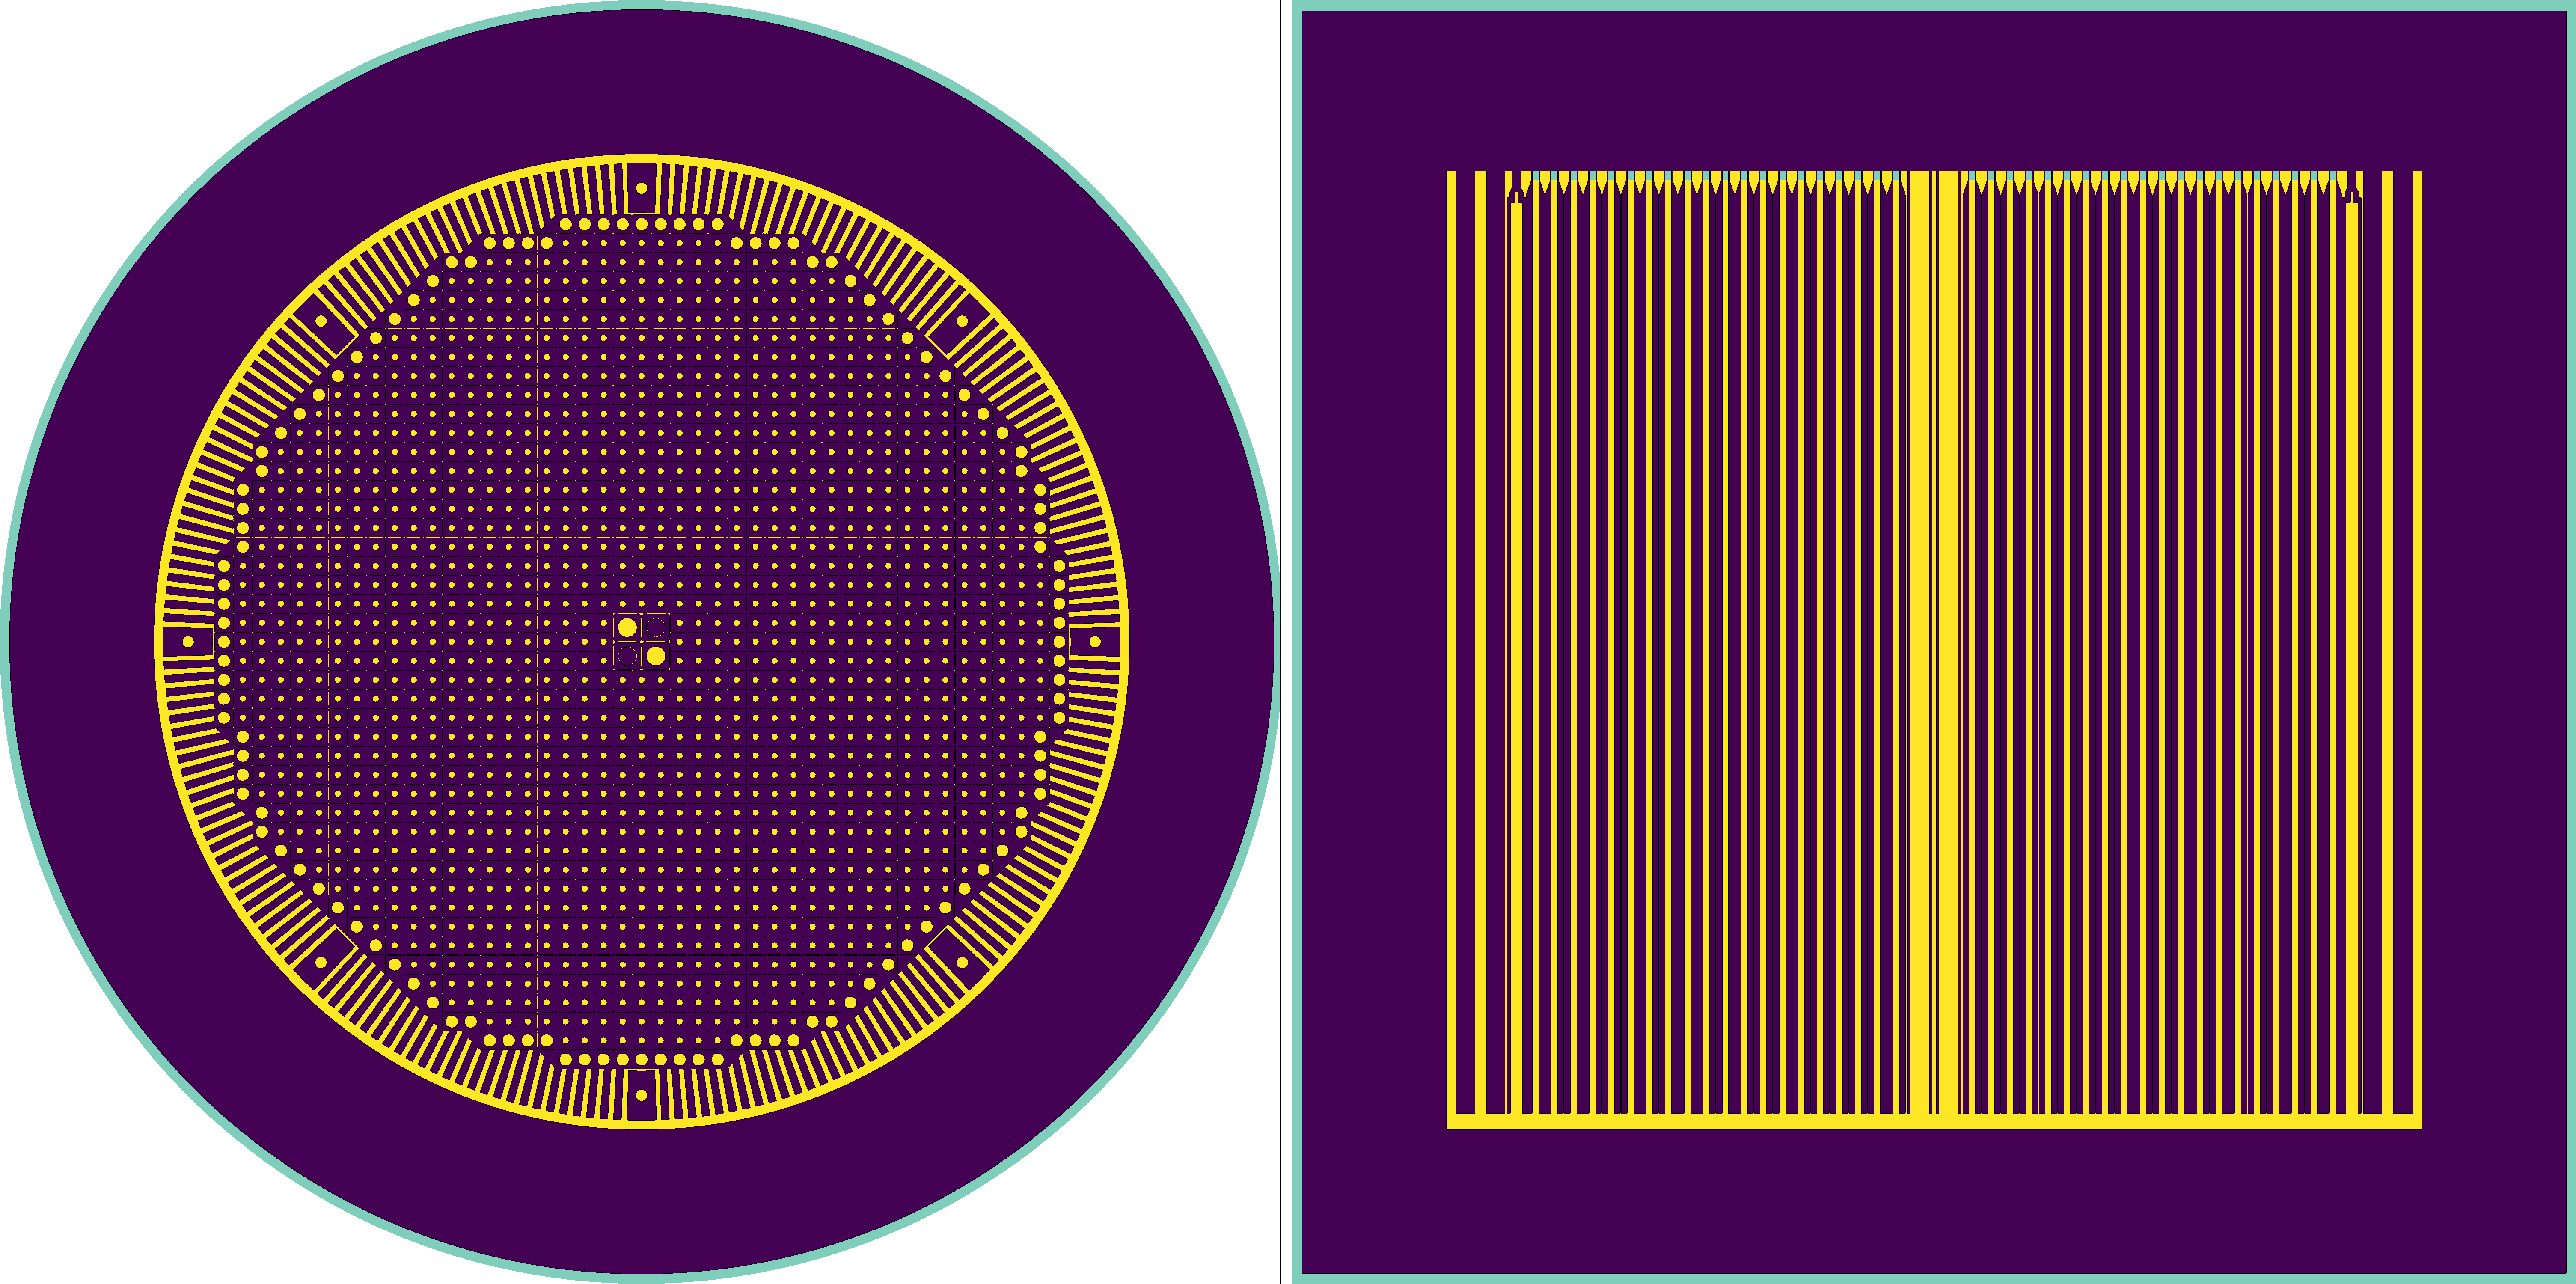
\includegraphics[width=\textwidth]{view_serpent.png}
  \caption{Plan and elevation views of SERPENT 2 \gls{MSBR} model developed in 
  this work.}
  \label{fig:serpent_plan_view}
\end{figure}

\begin{figure}[t!] % replace 't' with 'b' to \centering
  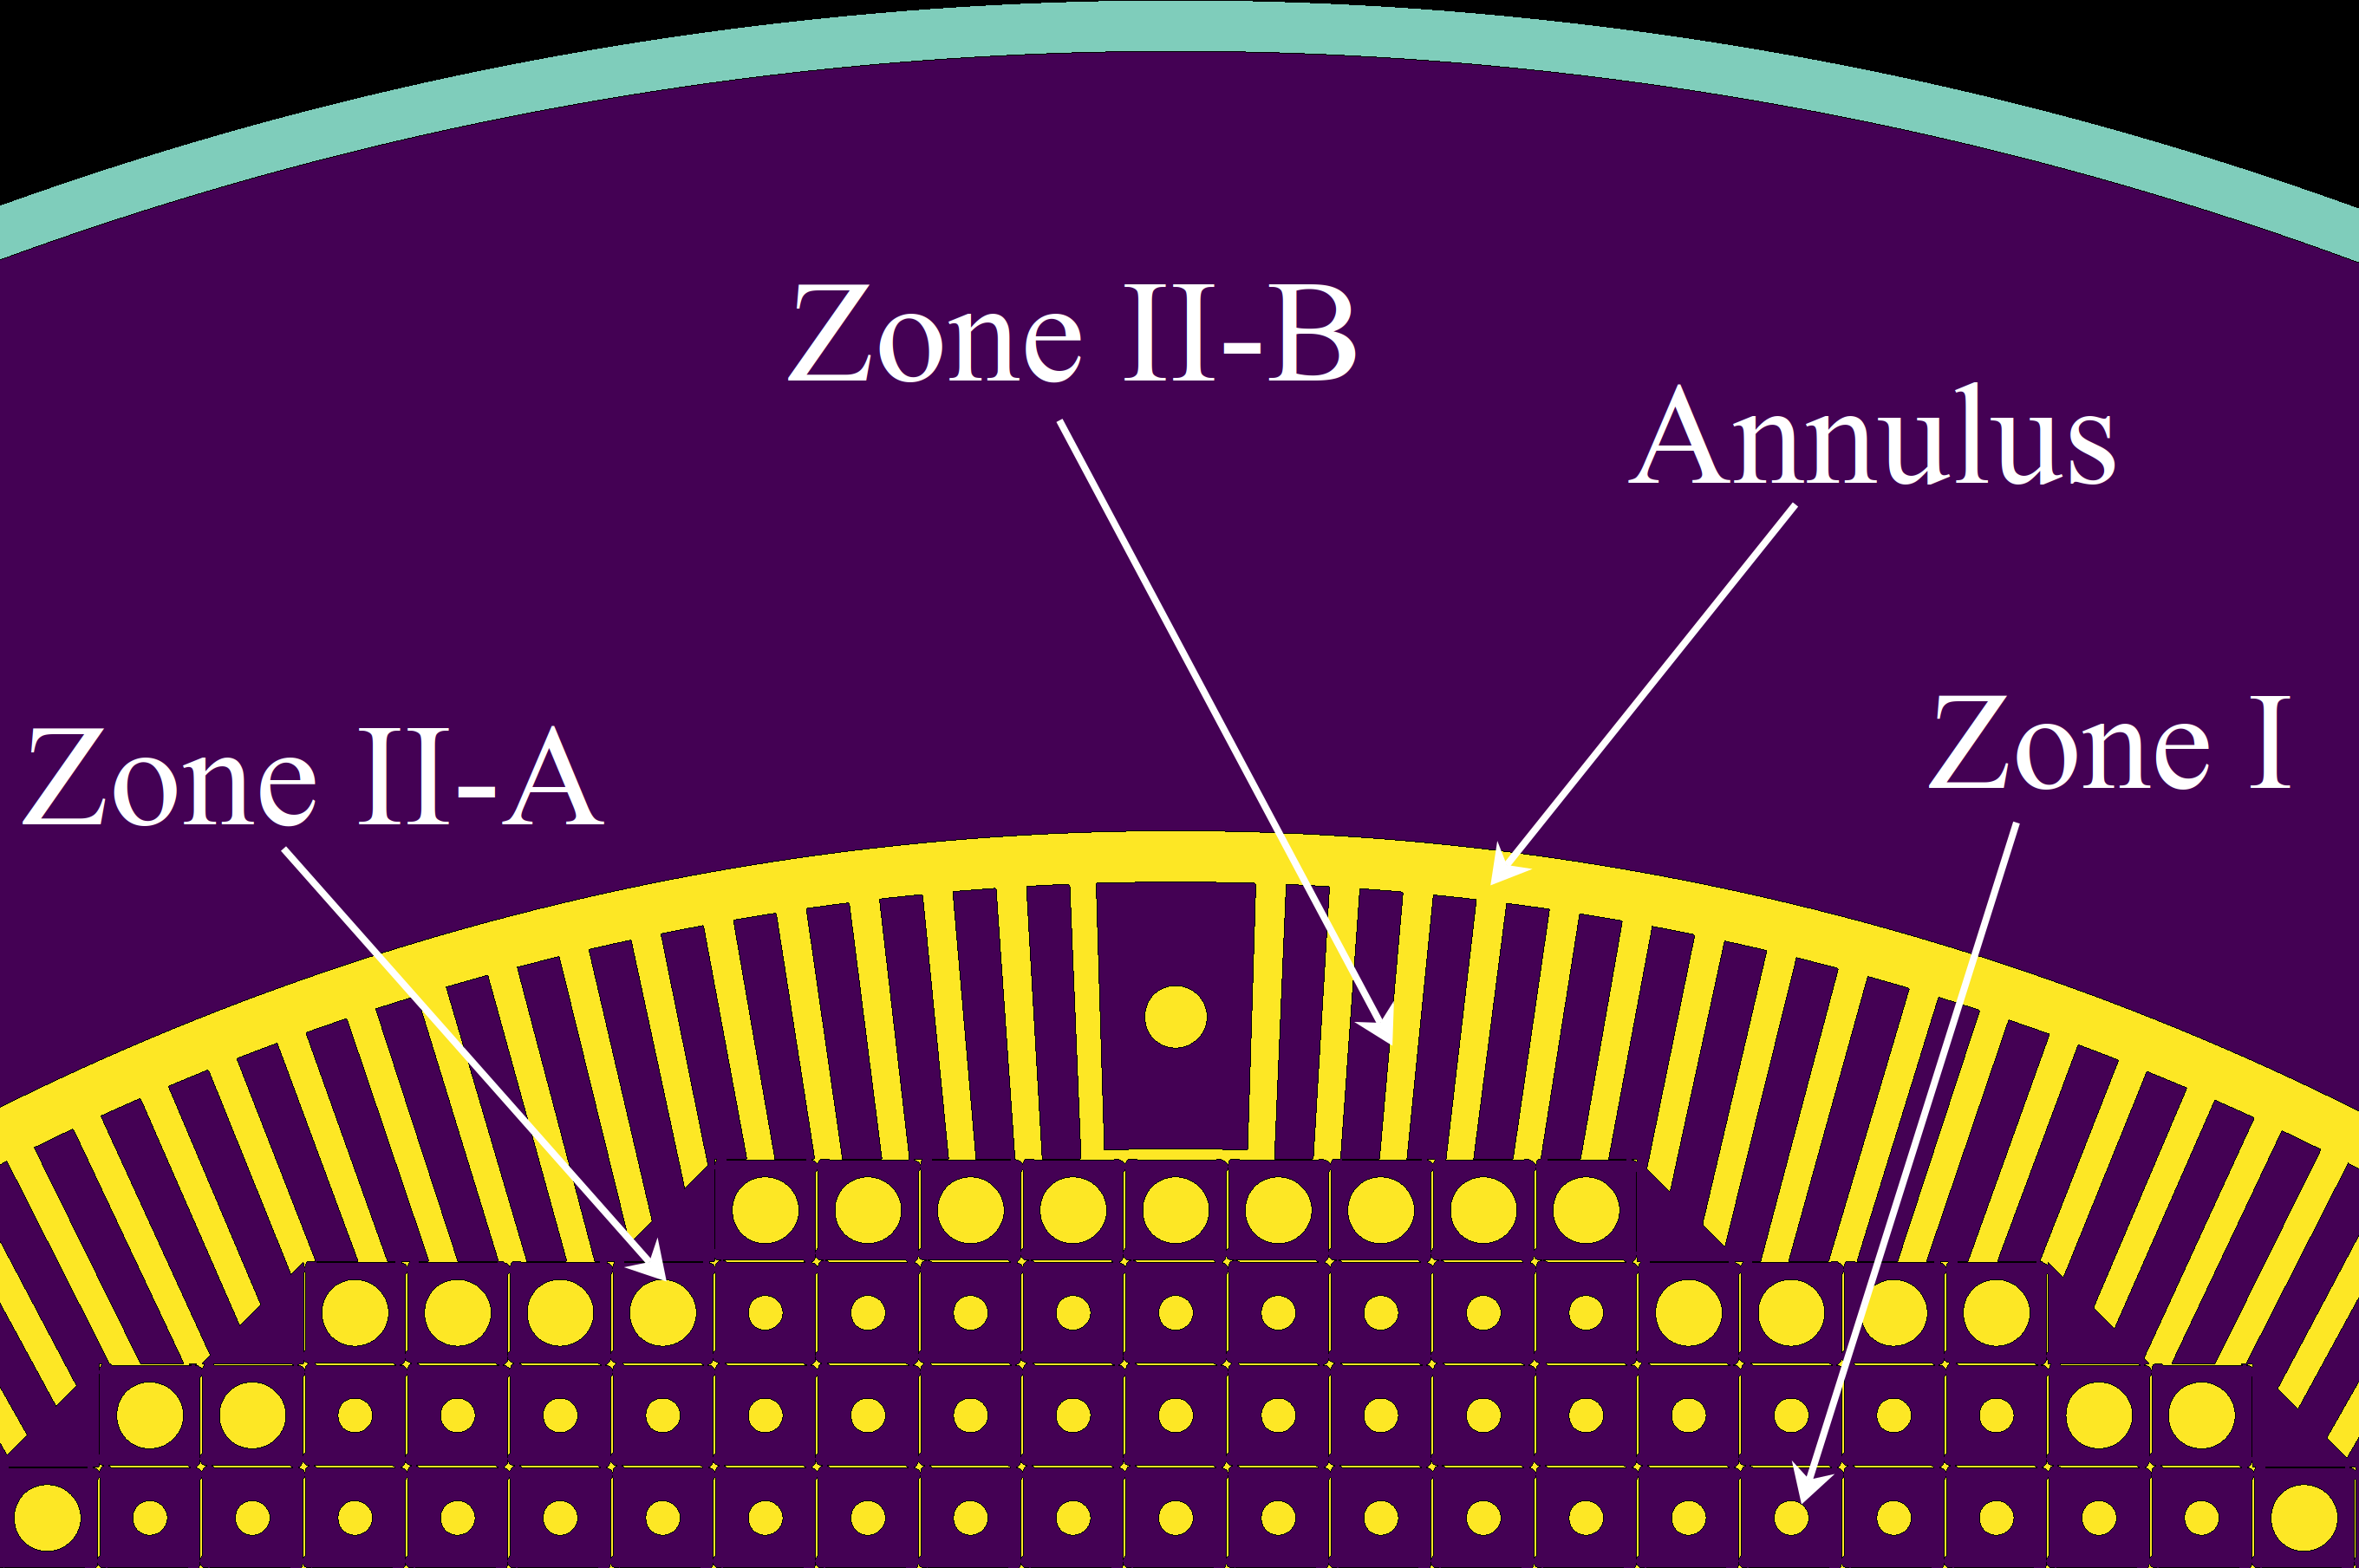
\includegraphics[width=\textwidth]{ser_zone_II.png}
  \caption{Detailed view of \gls{MSBR} two zone model. 
          Yellow represents fuel salt, purple represents graphite, and aqua represents the reactor vessel.}
  \label{fig:serpent_zoneII}
\end{figure}

Since reactor graphite experiences significant dimensional changes due to 
neutron irradiation, the reactor core was designed for periodic replacement. 
Based on the experimental irradiation data from the \gls{MSRE}, the core graphite 
lifetime is about 4 years and the reflector graphite lifetime is 30 years 
\cite{robertson_conceptual_1971}.

There are eight symmetric graphite slabs with a width of 15.24 cm in zone II, 
one of which is illustrated in Figure~\ref{fig:serpent_zoneII}. The holes in 
the centers are for the core lifting rods used during the core replacement 
operations. These holes also allow a portion of the fuel salt to flow to the 
top of the vessel for cooling the top head and axial reflector. 
Figure~\ref{fig:serpent_zoneII} also shows
the 5.08-cm-wide annular 
space between the removable core graphite in zone II-B and the permanently 
mounted reflector graphite. This annulus consists entirely of fuel salt, 
provides space for moving the core assembly, helps compensate for the elliptical 
dimensions of the reactor vessel, and serves to reduce the damaging flux at the 
surface of the graphite reflector blocks. 

$^{135}$Xe is a strong neutron poison, and some fraction of this gas 
is absorbed by graphite during \gls{MSBR} operation. ORNL calculations show 
that for unsealed commercial graphite with helium permeability 10$^{-5}$ 
cm$^2$/s the calculated poison fraction is less than 2\% 
\cite{robertson_conceptual_1971}.  This parameter can be improved by using 
experimental graphites or by applying sealing technology. The effect of the 
gradual poisoning of the core graphite with xenon is not treated here.

\subsubsection{Core zone I}
The central region of the core, called zone I, is made up of graphite elements, 
each $10.16$cm$\times$10.16cm$\times$396.24cm. Zone I has 4 channels for 
control rods: two for graphite rods which both regulate and shim during normal 
operation, and two for backup safety rods consisting of boron carbide clad to 
assure sufficient negative reactivity for emergency situations.

These graphite elements have a mostly rectangular shape with lengthwise ridges 
at each corner that leave space for salt flow elements. Various element sizes 
reduce the peak damage flux and power density in the center of the core to 
prevent local graphite damage.  Figure~\ref{fig:I_element_ref} shows the 
elevation and plan views of graphite elements of zone I 
\cite{robertson_conceptual_1971} and their SERPENT model 
\cite{rykhlevskii_full-core_2017}.

\begin{figure}[ht!] % replace 't' with 'b' to \centering
  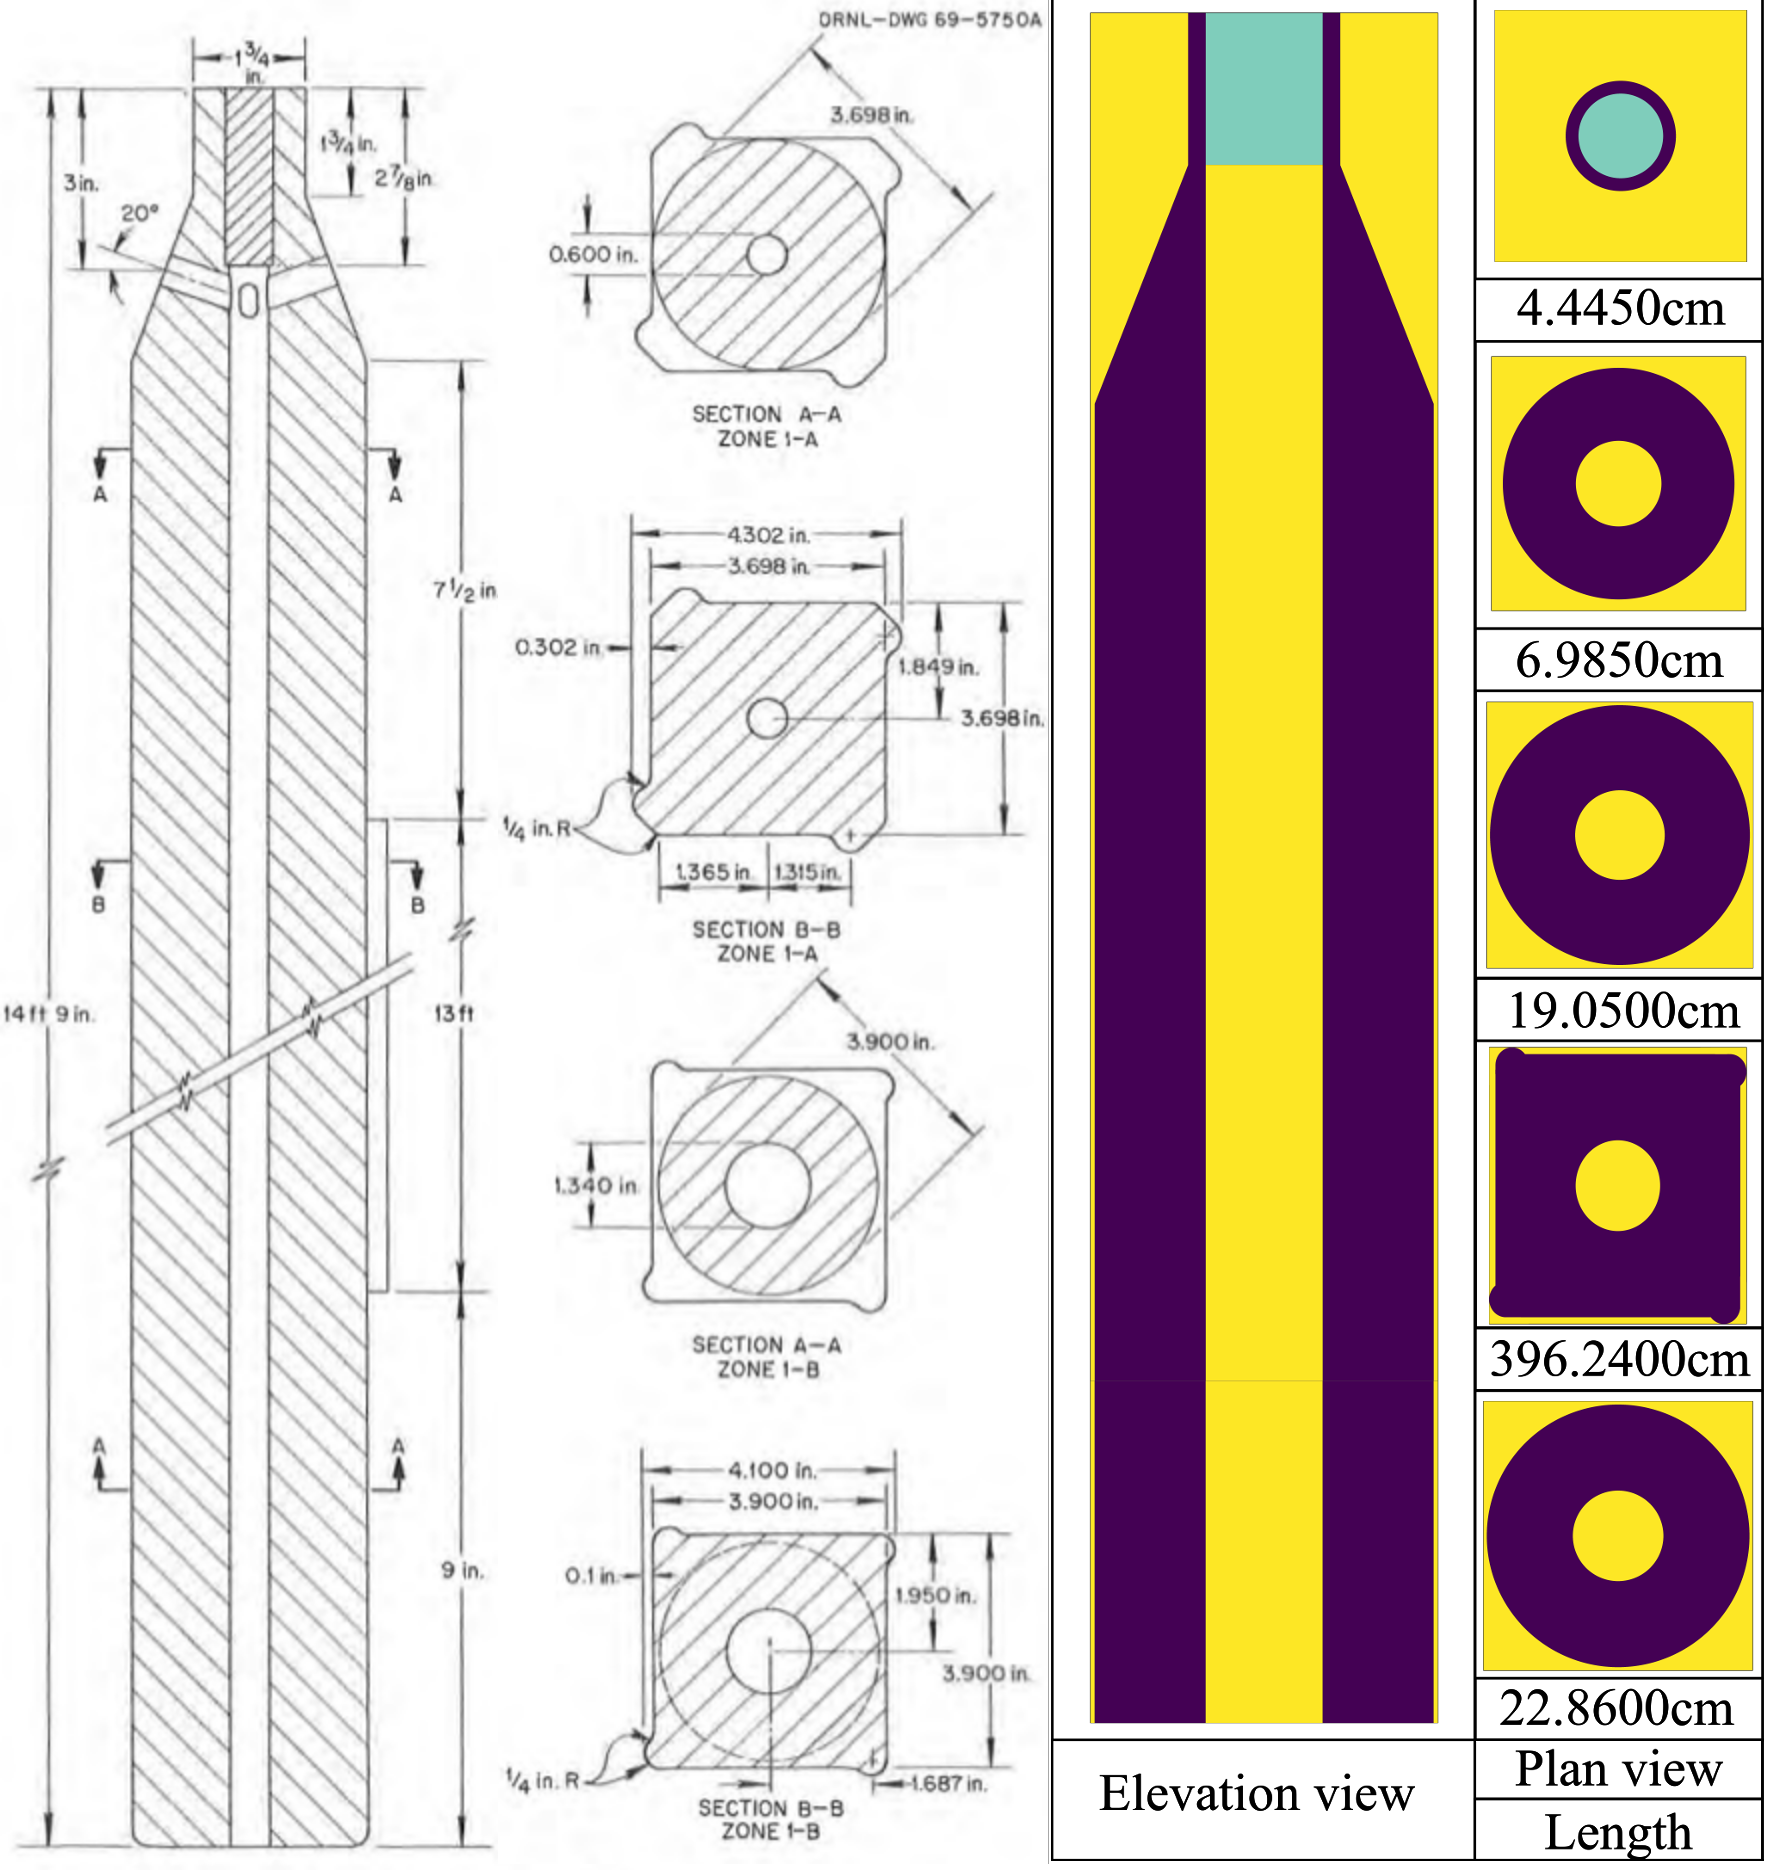
\includegraphics[width=\textwidth]{zone_I_element_ref.png}
  \caption{Graphite moderator elements for zone I 
  \cite{robertson_conceptual_1971,rykhlevskii_full-core_2017}.  Yellow 
  represents fuel salt, purple represents graphite, and aqua represents the 
  reactor vessel.}
  \label{fig:I_element_ref}
\end{figure}

\subsubsection{Core zone II}
Zone II, which is undermoderated, surrounds zone I. Combined with the bounding 
radial reflector, zone II serves to diminish neutron leakage. Two kinds of 
elements form this zone: large-diameter fuel channels (zone II-A) and 
radial graphite slats (zone II-B). 

Zone II has 37\% fuel salt by volume and each element has a fuel channel 
diameter of 6.604cm. The graphite elements for zone II-A are prismatic with
elliptical dowels running axially between the prisms. These dowels
isolate the fuel salt flow in zone I from that in zone II. 
Figure~\ref{fig:II_element_ref} shows the shapes and dimensions of these graphite 
elements and their SERPENT model. Zone II-B elements are rectangular slats 
spaced far enough apart to provide the 0.37 fuel salt volume fraction. The 
reactor zone II-B graphite 5.08cm-thick slats vary in the radial dimension 
(average width is 26.67cm) as shown in figure~\ref{fig:serpent_zoneII}. Zone II 
serves as a blanket to achieve the best performance: a high breeding ratio and 
a low fissile inventory. The harder neutron energy spectrum in zone II 
enhances the rate of thorium resonance capture relative to the fission rate, 
thus limiting the neutron flux in the outer core zone and reducing the neutron 
leakage \cite{robertson_conceptual_1971}. 

The sophisticated, irregular shapes of the fuel elements challenge an accurate 
representation of zone II-B.  
The suggested design \cite{robertson_conceptual_1971} of zone II-B has 8 
irregularly-shaped graphite elements as well as dozens of salt channels. 
These graphite elements were simplified into right-circular cylindrical shapes  
with central channels. Figure~\ref{fig:serpent_zoneII} illustrates this core 
region in the SERPENT model. The volume of fuel salt in zone II was kept 
exactly at 37\%, so that this simplification did not considerably change the core 
neutronics. Simplyfying the eight edge channels was the only simplification made 
to the \gls{MSBR} geometry in this work. 

\begin{figure}[ht!] % replace 't' with 'b' to \centering
  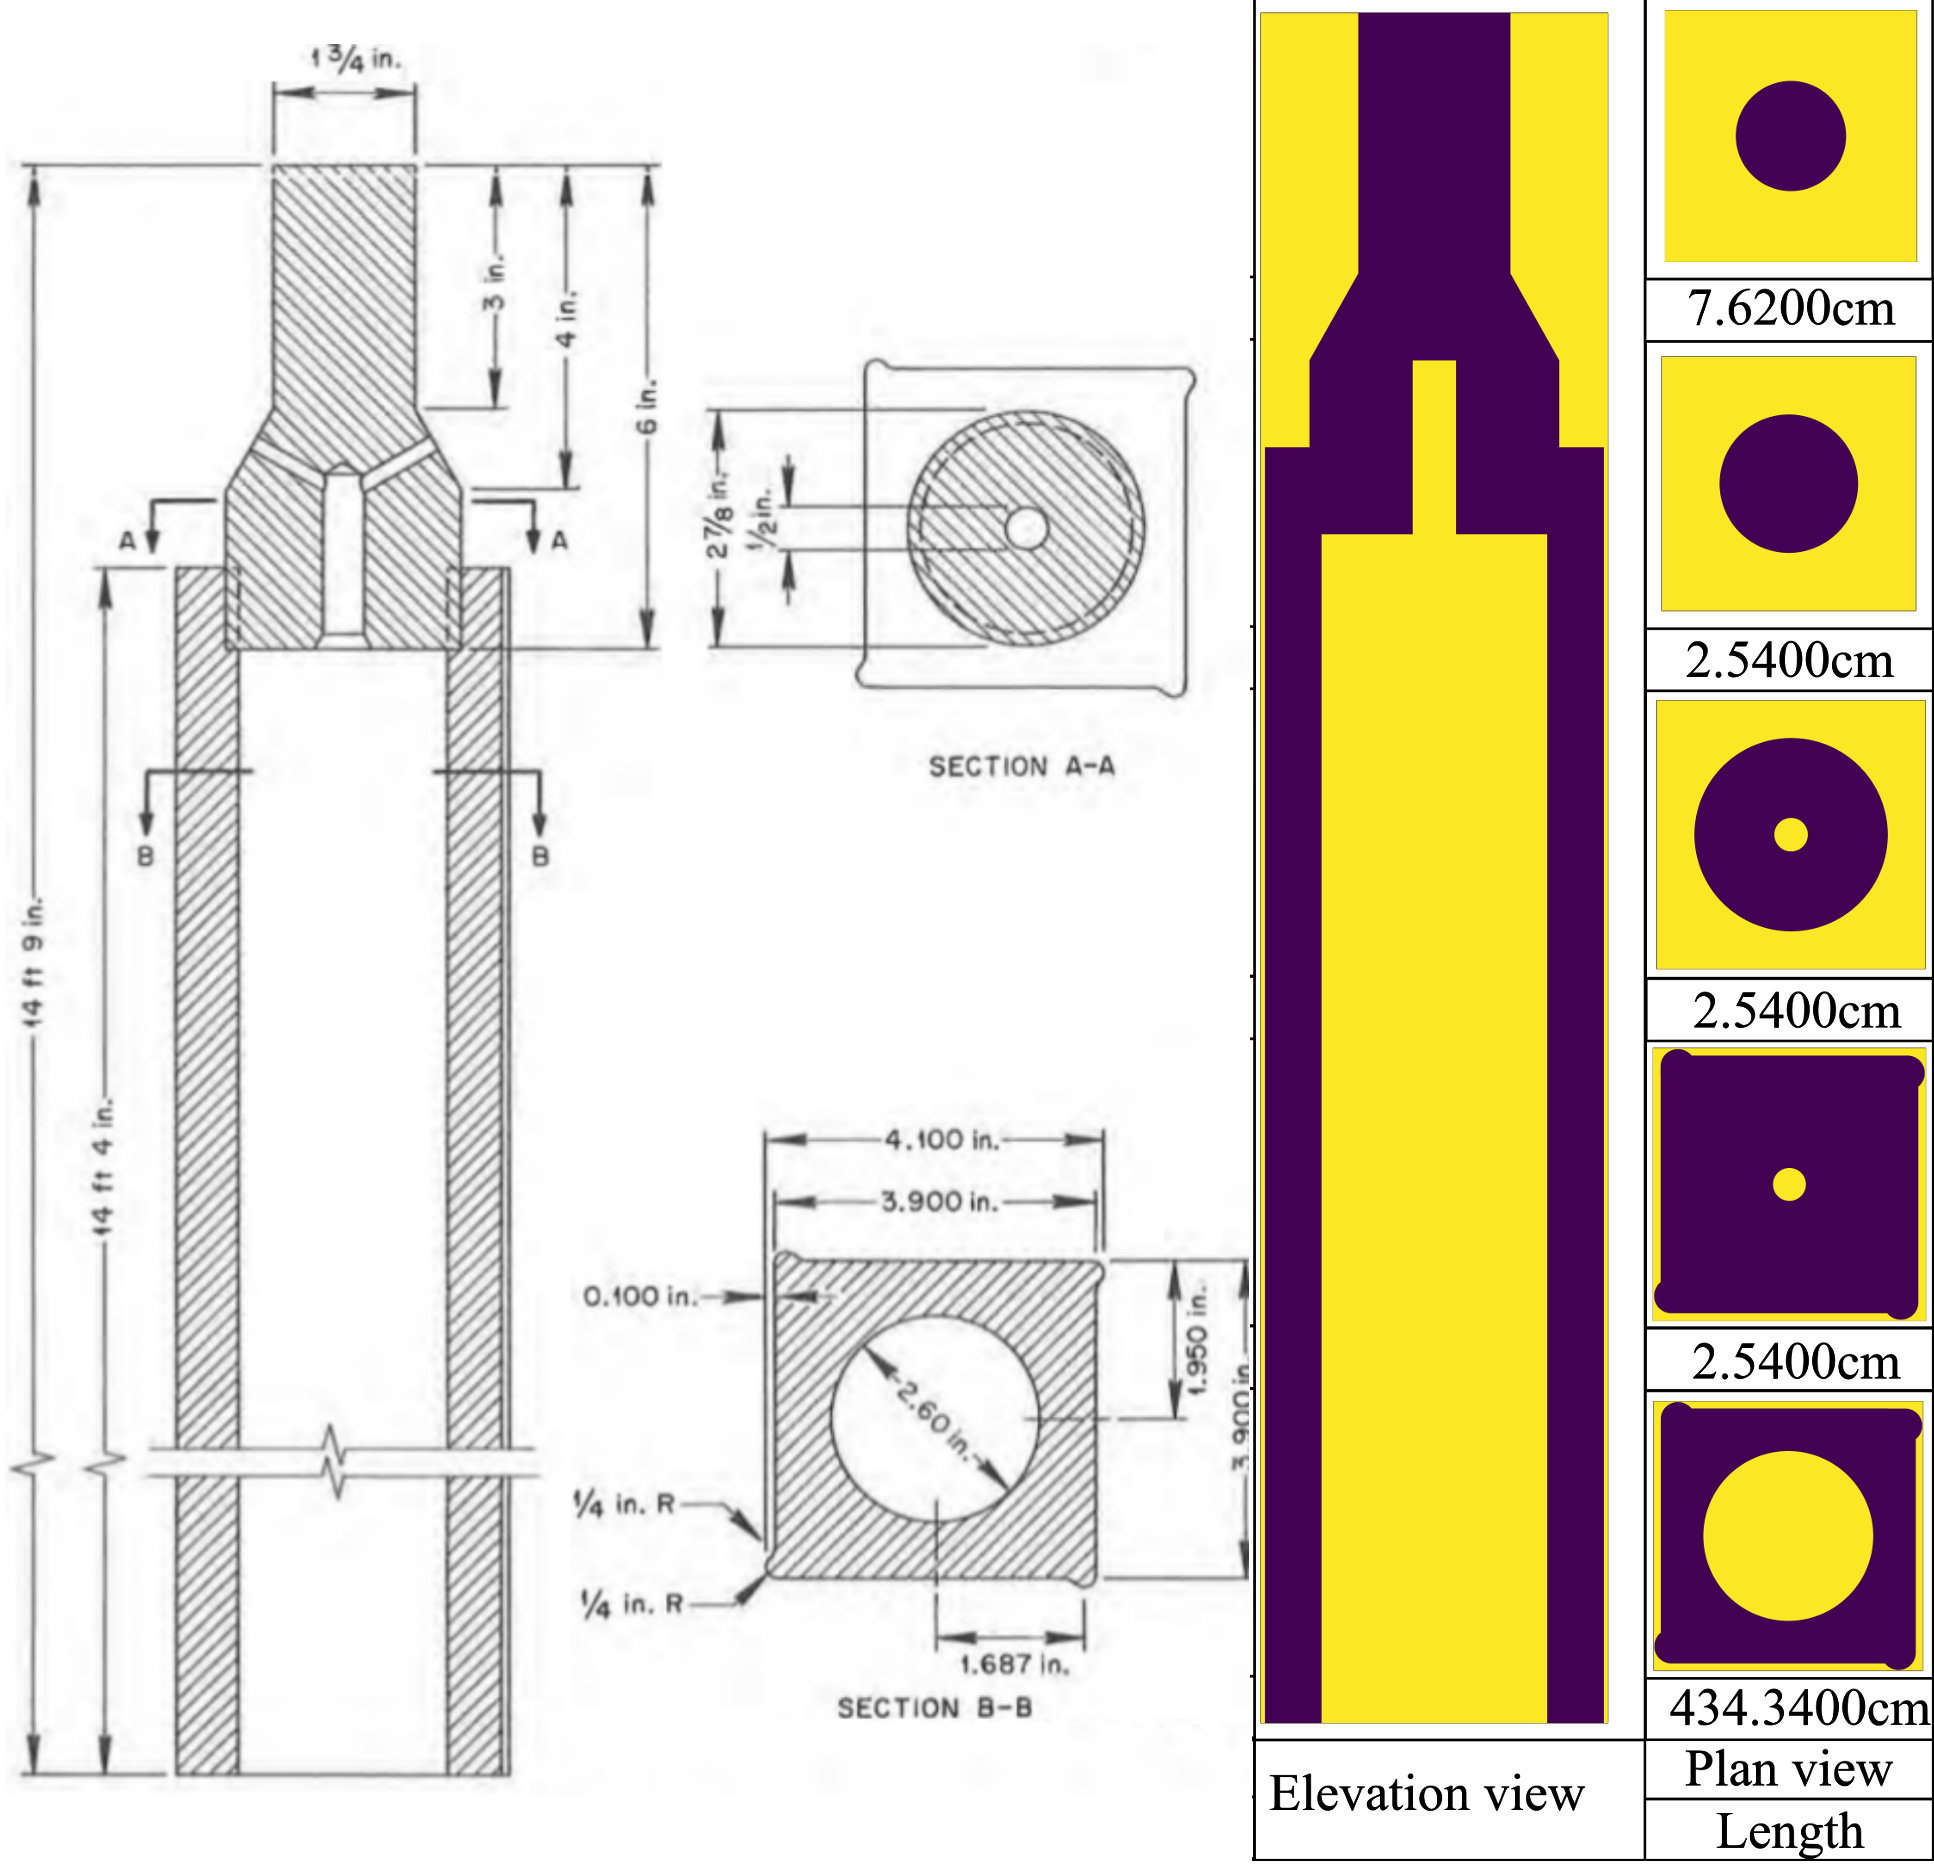
\includegraphics[width=\textwidth]{zone_II_element_ref.png}
  \caption{Graphite moderator elements for zone II-A 
  \cite{robertson_conceptual_1971,rykhlevskii_full-core_2017}.  Yellow 
  represents fuel salt and purple represents graphite.}
  \label{fig:II_element_ref}
\end{figure}

\subsubsection{Material composition and normalization parameters}
The fuel salt, reactor graphite, and modified Hastelloy-N
are all materials created at \gls{ORNL} specifically for the \gls{MSBR}.
The initial fuel salt used the same 
density (3.35 g/cm$^3$) and composition LiF-BeF$_2$-ThF$_4$-$^{233}$UF$_4$ 
(71.75-16-12-0.25 mole \%) as the \gls{MSBR} design 
\cite{robertson_conceptual_1971}. The lithium in the molten salt fuel is fully 
enriched to 100\% $^{7}$Li because $^{6}$Li is a very strong neutron poison and 
becomes tritium upon neutron capture. 

The JEFF-3.1.2 neutron library provided cross section generation 
\cite{oecd/nea_data_bank_jeff-3.1.2_2014}. 
The specific temperature was fixed for each material and did not change during 
the reactor operation. The isotopic 
composition of each material at the initial state was described in detail in 
the MSBR conceptual design study \cite{robertson_conceptual_1971} and has been 
applied to the SERPENT model without any modification. Table~\ref{tab:msbr_tab} is 
a summary of the major \gls{MSBR} parameters used by this model 
\cite{robertson_conceptual_1971}. 

%%%%%%%%%%%%%%%%%%%%%%%%%%%%%%%%%%%%%%%%
\begin{table}[h!]
        \caption{Summary of principal data for \gls{MSBR} 
        \cite{robertson_conceptual_1971}.}
        \begin{tabularx}{\textwidth}{ s  s}
        \hline
                Thermal capacity of reactor           		& 2250 MW(t)
                \\ Net electrical output                 		& 1000 
        MW(e) \\  Net thermal efficiency        				
        & 44.4\%
                \\  Salt volume fraction in central zone I		& 0.13
                \\ Salt volume fraction in outer zone II       & 0.37
                \\ Fuel salt inventory (Zone I)                & 8.2 m$^3$	
        \\ Fuel salt inventory (Zone II)               & 10.8 m$^3$	\\ Fuel 
        salt inventory (annulus)               & 3.8 m$^3$	\\  Total fuel 
        salt inventory                   & 48.7 m$^3$	\\ Fissile mass in fuel 
        salt                   & 1303.7 kg	\\ Fuel salt components                  
                               & LiF-BeF$_2$-ThF$_4$-$^{233}$UF$_4$	\\  
        Fuel salt composition                 & 71.75-16-12-0.25 mole\%
                \\
                Fuel salt density                    & 3.35 g/cm$^3$
                \\ \hline
        \end{tabularx}
        \label{tab:msbr_tab}
\end{table}
%%%%%%%%%%%%%%%%%%%%%%%%%%%%%%%%%%%%%%%%%%%%%%%%

\subsection{Online reprocessing method}
Removing specific chemical elements from a molten salt 
requires intelligent design (e.g., chemical separations equipment design, 
fuel salt flows to equipment) and has a considerable economic cost. All 
liquid-fueled \gls{MSR} designs involve varying levels of online fuel 
processing. Minimally, volatile gaseous fission products (e.g. Kr, Xe) escape 
from the fuel salt during routine reactor operation and must be captured. 
Additional systems might be used to enhance removal of those elements. Most 
designs also call for the removal of noble and rare earth metals from the core 
since these metals act as neutron poisons. Some designs suggest a more complex 
list of elements to process (figure~\ref{fig:periodic_tab}), including the 
temporary removal of protactinium or other regulation of the 
actinide inventory \cite{ahmad_neutronics_2015}.

\begin{figure}[htp!] % replace 't' with 'b' to \centering
  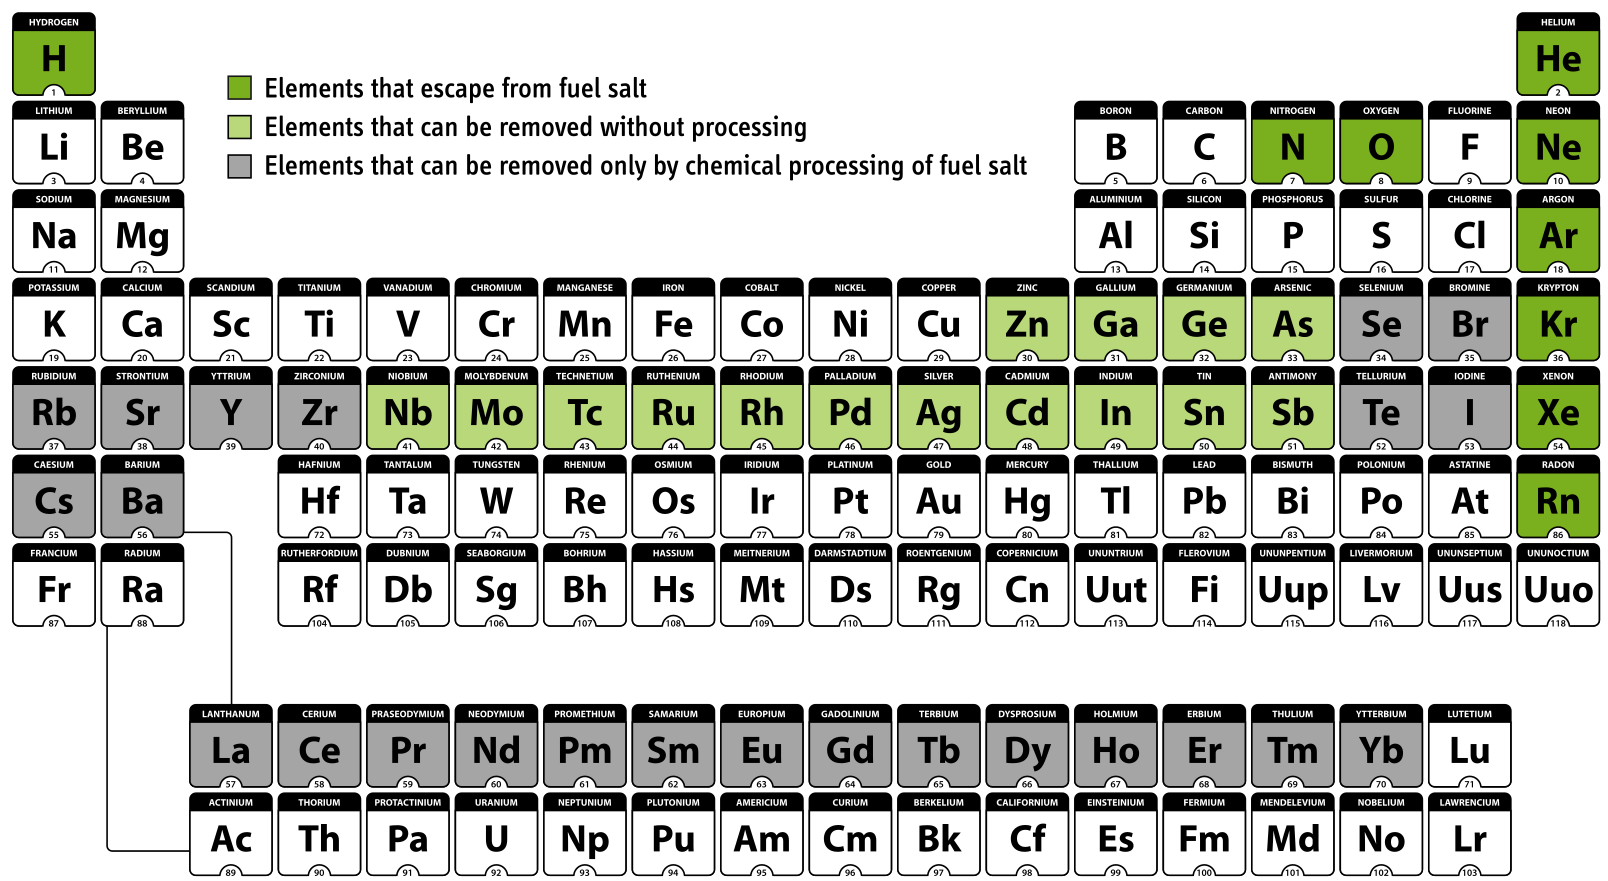
\includegraphics[width=\textwidth]{periodic_map.png}
  \caption{Processing options for \gls{MSR} fuels. 
          Reproduced from \cite{ahmad_neutronics_2015} where it was adapted 
          from a chart courtesy of Nicolas 
          Raymond, www.freestock.ca.}
  \label{fig:periodic_tab}
\end{figure}

\subsubsection{Fuel material flows}
The $^{232}$Th in the fuel absorbs thermal neutrons and produces $^{233}$Pa 
which then decays into the fissile $^{233}$U. Furthermore, the \gls{MSBR} 
design requires online reprocessing to remove all poisons (e.g. $^{135}$Xe), 
noble metals, and gases (e.g. $^{75}$Se, $^{85}$Kr) every 20 seconds. 
Protactinium presents a challenge, since it has a large absorption cross 
section in the thermal energy spectrum. Moreover, $^{233}$Pa left in the core
would produce $^{234}$Pa and $^{234}$U, neither of which are useful as fuel. 
Accordingly, $^{233}$Pa is continuously 
removed from the fuel salt into a protactinium decay tank to allow $^{233}$Pa 
to decay to $^{233}$U without the corresponding negative neutronic impact. The reactor 
reprocessing system must separate $^{233}$Pa from the molten-salt fuel over 3 
days, hold it while $^{233}$Pa decays into $^{233}$U, and return it back to the 
primary loop. This feature allows the reactor to avoid neutron losses to 
protactinium, lowers in-core fission product inventory, and increases the 
efficiency of $^{233}$U breeding. Table~\ref{tab:reprocessing_list} summarizes 
full list of nuclides and the ``cycle times''\footnote{ The \gls{MSBR} program defined a ``cycle time" as the amount of time required to remove 100\% of a target nuclide from a fuel 
salt \cite{robertson_conceptual_1971}.} used for modeling salt treatment and 
separations \cite{robertson_conceptual_1971}. 

%%%%%%%%%%%%%%%%%%%%%%%%%%%%%%%%%%%%%%%%
\begin{table}[ht!]
        \caption{The effective cycle times for protactinium and fission 
        products removal (reproduced from \cite{robertson_conceptual_1971}).}
        \begin{tabularx}{\textwidth}{ x | s | x }
        \hline Processing group & \qquad\qquad\qquad Nuclides & Cycle time (at 
                full power) \\ \hline Rare earths & Y, La, Ce, Pr, Nd, Pm, Sm, 
                Gd & 50 days \\ \qquad & Eu & 500 days \\ Noble metals & Se, 
                Nb, Mo, Tc, Ru, Rh, Pd, Ag, Sb, Te & 20 sec \\
        Seminoble metals & Zr, Cd, In, Sn & 200 days \\
        Gases & Kr, Xe & 20 sec \\ Volatile fluorides & Br, I & 60 days \\
        Discard & Rb, Sr, Cs, Ba & 3435 days \\ 
        %Salt discard & Th, Li, Be, F & 3435 days \\ 
        Protactinium & $^{233}$Pa & 3 days \\ Higher 
                nuclides & $^{237}$Np, $^{242}$Pu & 16 years \\  \hline
        \end{tabularx}
        \label{tab:reprocessing_list}
\end{table}
The removal rates vary among nuclides in this reactor concept which dictate the 
necessary resolution of depletion calculations. If the depletion time intervals 
are very short, an enormous number of depletion steps are required to obtain 
the equilibrium composition. On the other hand, if the depletion  calculation 
time interval is too long, the impact of short-lived fission products is not 
captured. To compromise, a 3 day time interval was selected for depletion 
calculations\footnote{ Optimal depletion time step of 3 days for \gls{MSR} 
batch-wise depletion simulation was first described and concluded by Powers 
\emph{et al.} \cite{powers_new_2013}.} to correlate with the removal interval 
of 
$^{233}$Pa and $^{232}$Th was continuously added to maintain the initial mass 
fraction of $^{232}$Th.
\FloatBarrier
\section{Results}


\subsection{Effective multiplication factor}
Figures~\ref{fig:keff}, \ref{fig:keff_zoomed} show the effective multiplication factors. 

\begin{figure}[ht!] 
  \centering
  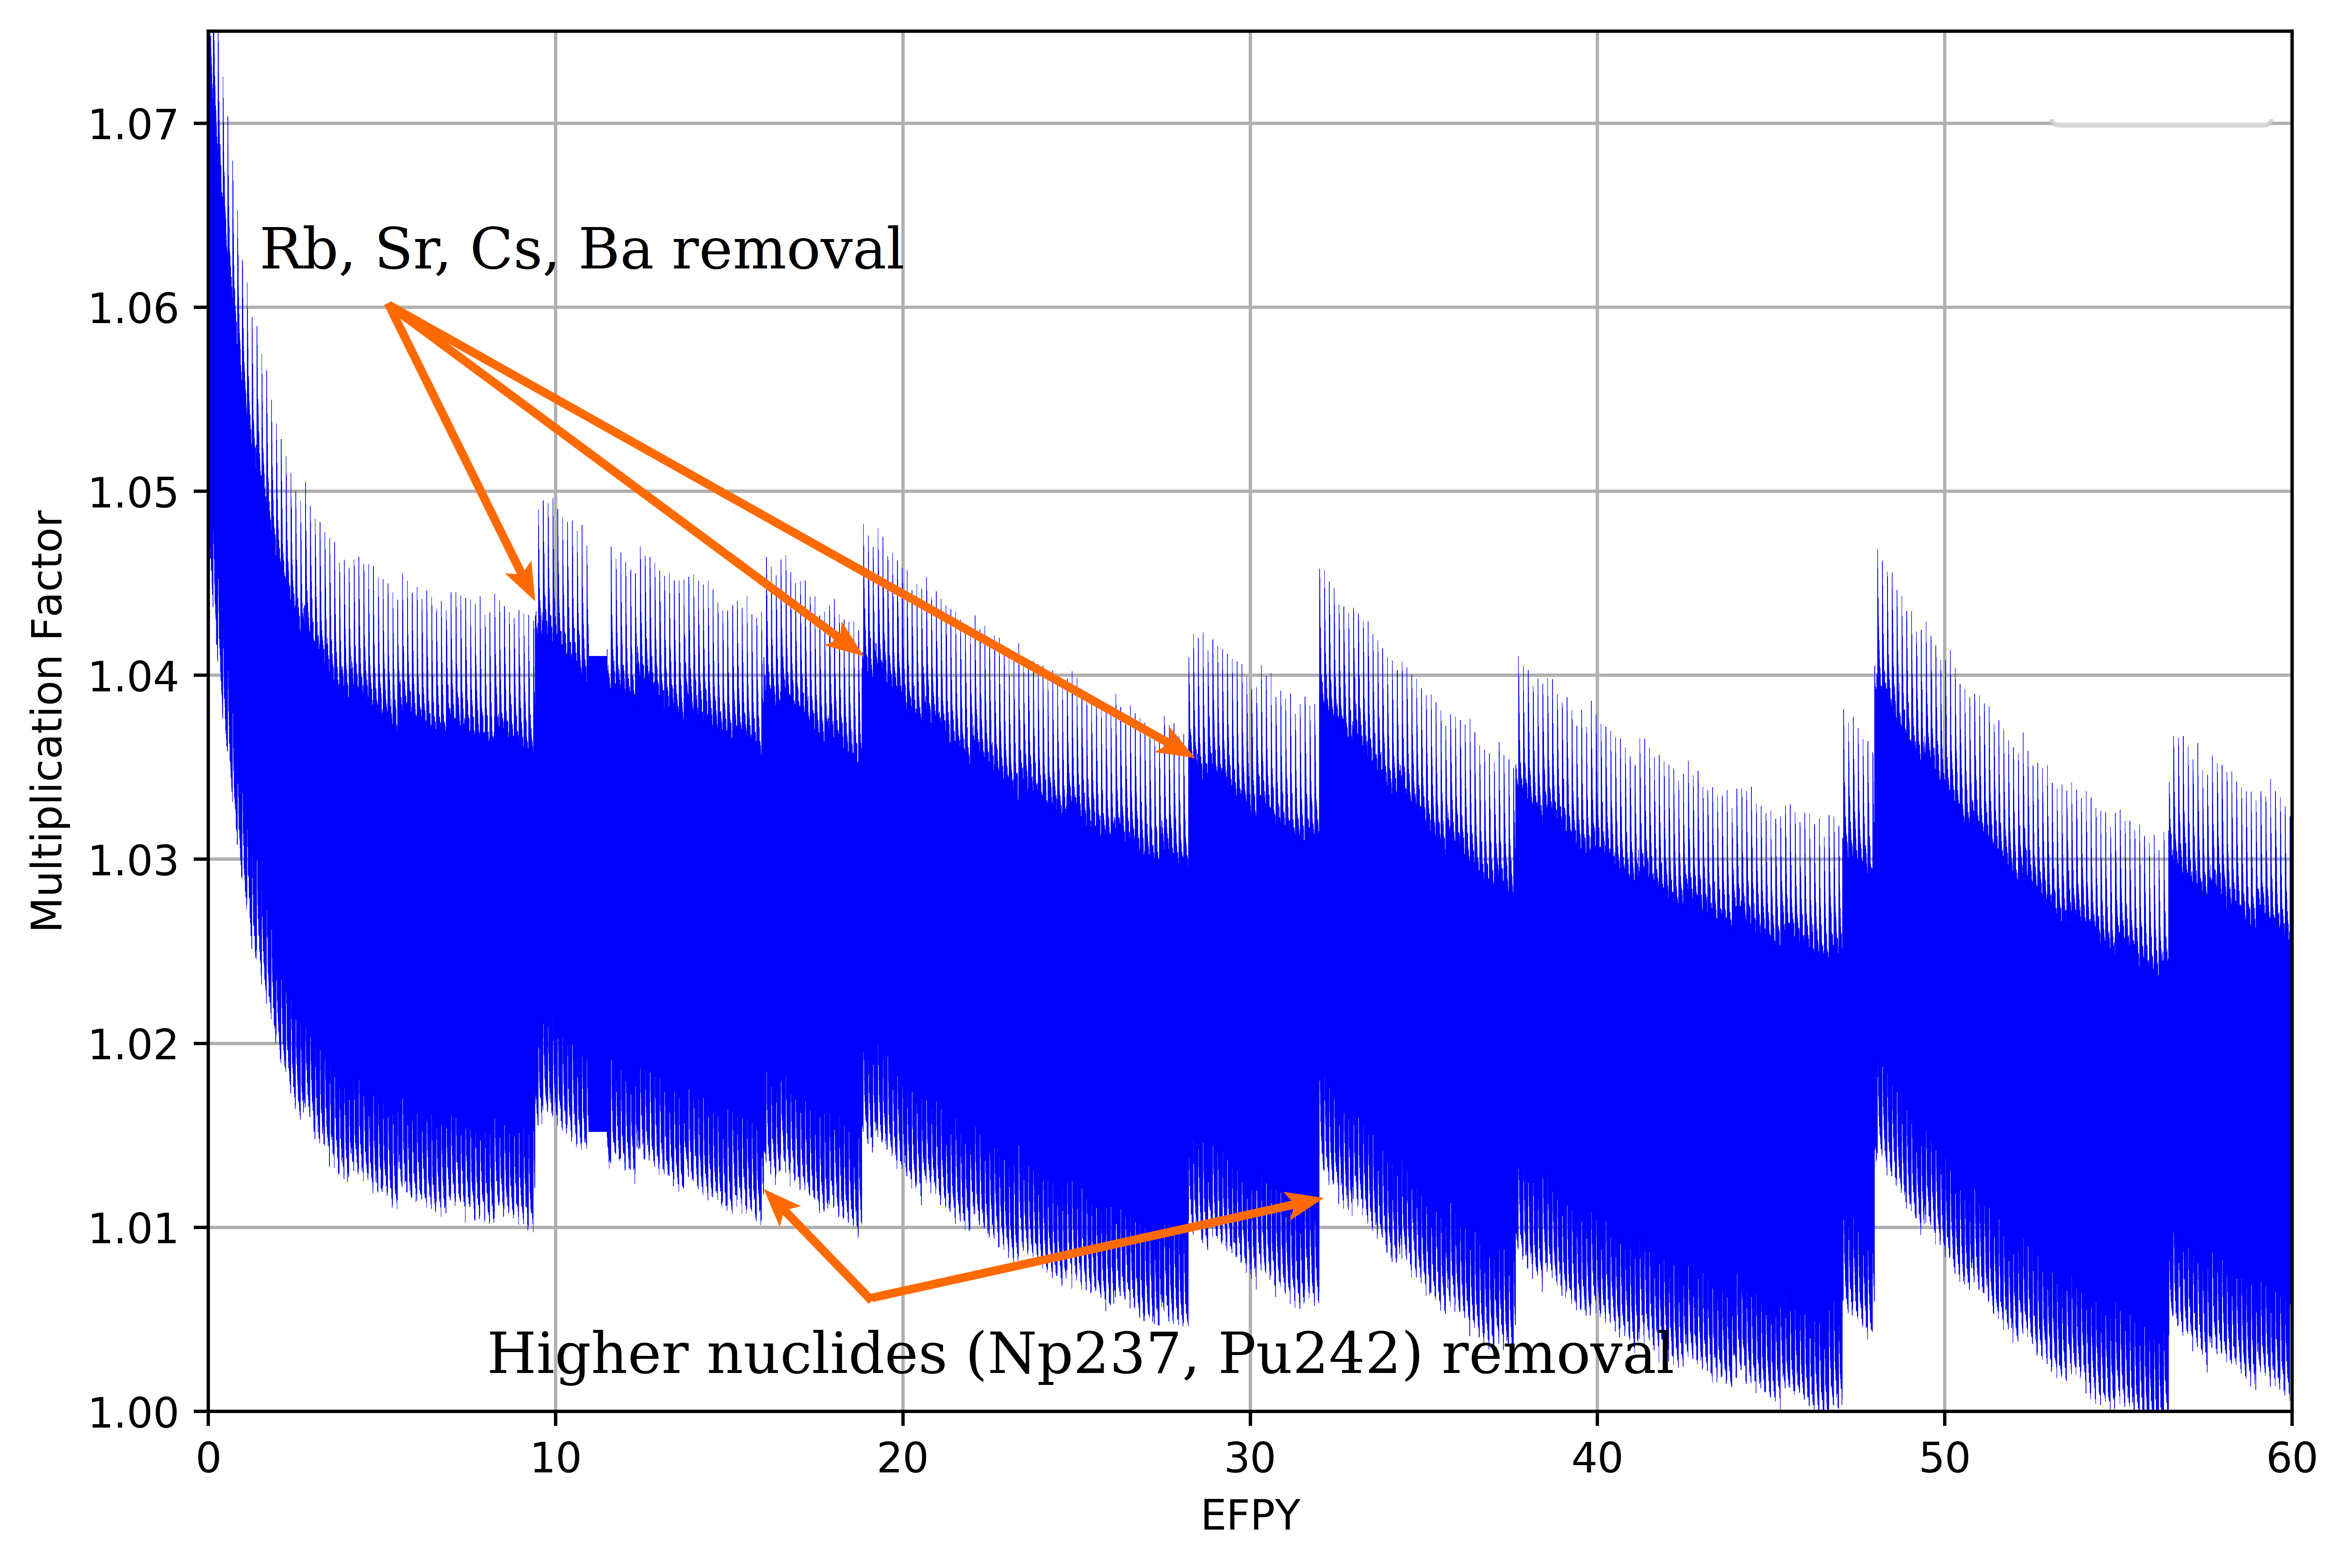
\includegraphics[width=\textwidth]{keff.png}
  \caption{Effective multiplication factor dynamics for full-core \gls{MSBR} 
  model over a 60-year reactor operation lifetime.}
  \label{fig:keff}
\end{figure}
\begin{figure}[ht!] 
  \centering
  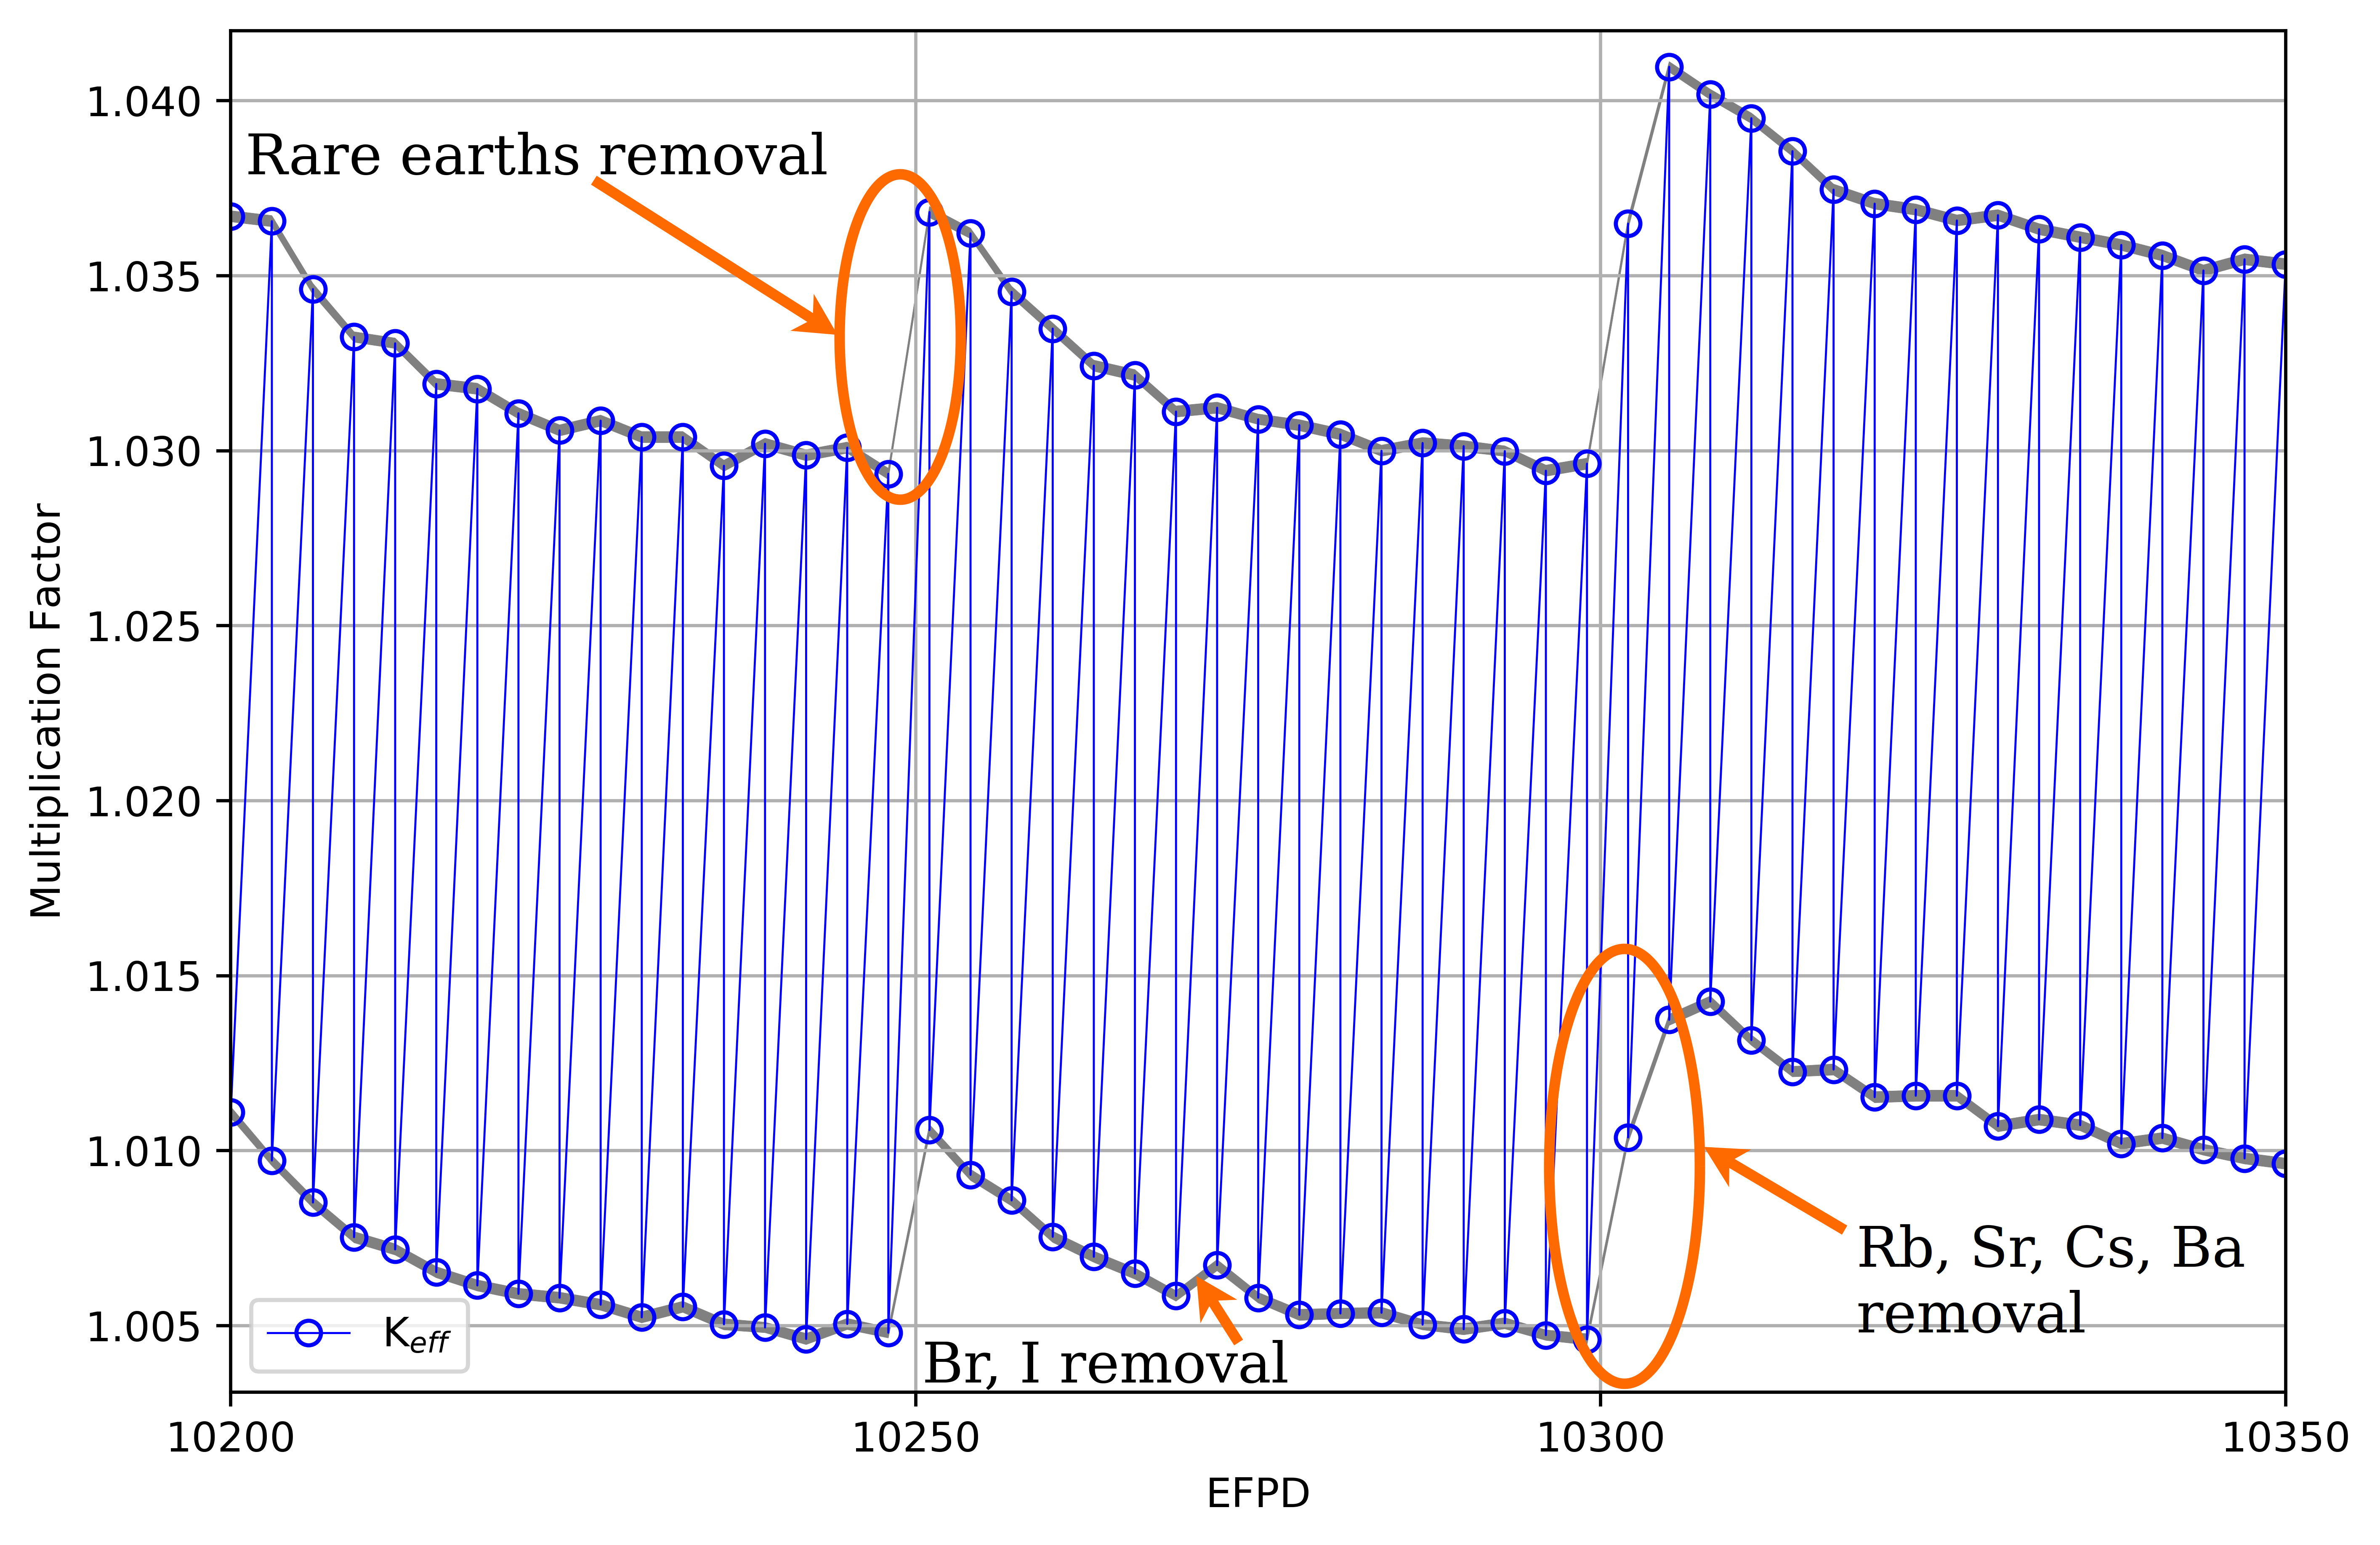
\includegraphics[width=\textwidth]{keff_zoomed.png}
  \caption{Zoomed effective multiplication factor for 150-EFPD time interval.}
  \label{fig:keff_zoomed}
\end{figure}

\subsection{Fuel salt composition dynamics}
The analysis of the fuel salt composition evolution provides more comprehensive 
information about the equilibrium state. Figure~\ref{fig:adens_eq} shows the number 
densities of major nuclides which have a strong influence on the reactor core 
physics. The concentration of $^{233}$U, $^{232}$Th, $^{233}$Pa, and $^{232}$Pa in 
the fuel salt change insignificantly after approximately 2500 days of operation. 
In particular, the $^{233}$U number density fluctuates by less than 0.8\% between
 16 and 20 years of operation. Hence, a quasi-equilibrium state was 
achieved after 16 years of reactor operation.
\begin{figure}[ht!] % replace 't' with 'b' to 
  \centering
  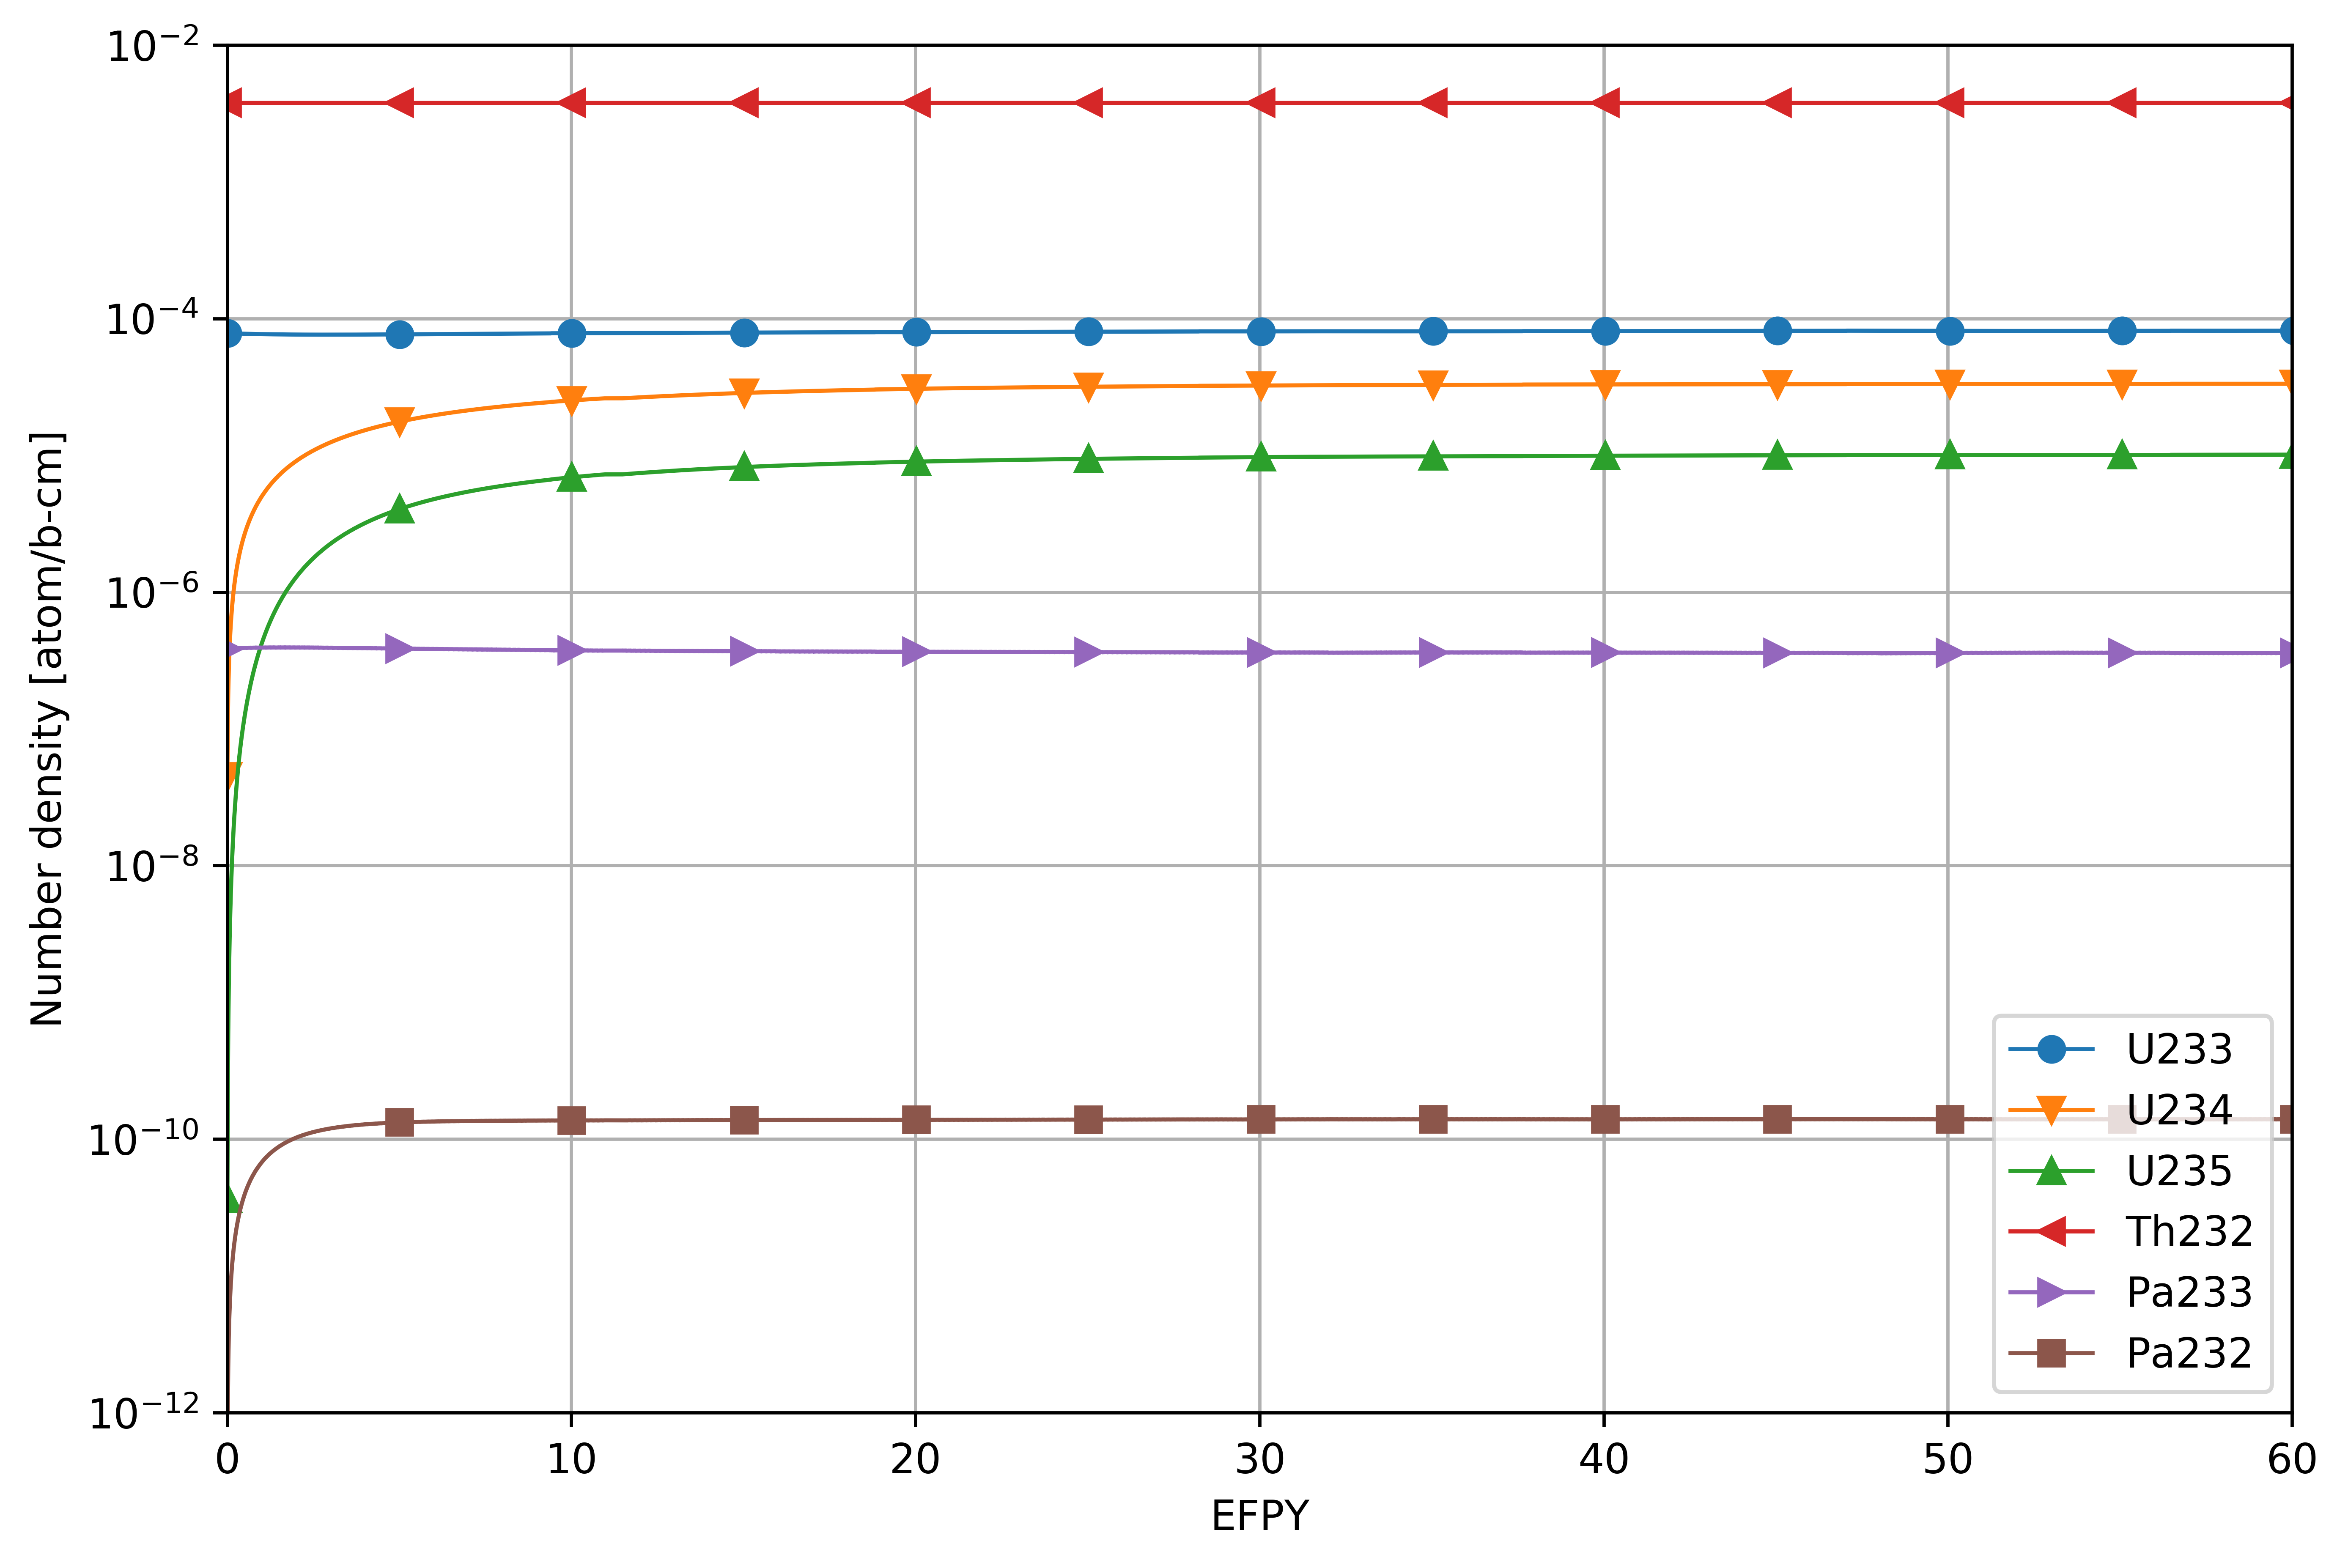
\includegraphics[width=\textwidth]{major_isotopes_adens.png}
  \caption{Number density of major nuclides during 60 years of reactor 
  operation.}
  \label{fig:adens_eq}
\end{figure}

\subsection{Neutron spectrum}
Figure~\ref{fig:spectrum} shows the normalized neutron flux spectrum for the 
full-core \gls{MSBR} model in the energy range from $10^{-8}$ to $10$ MeV. The 
neutron energy spectrum at equilibrium is harder than at startup due to 
plutonium and other strong absorbers accumulating in the core during reactor 
operation.  
\begin{figure}[ht!] % replace 't' with 'b'         to force it to 
  \centering
  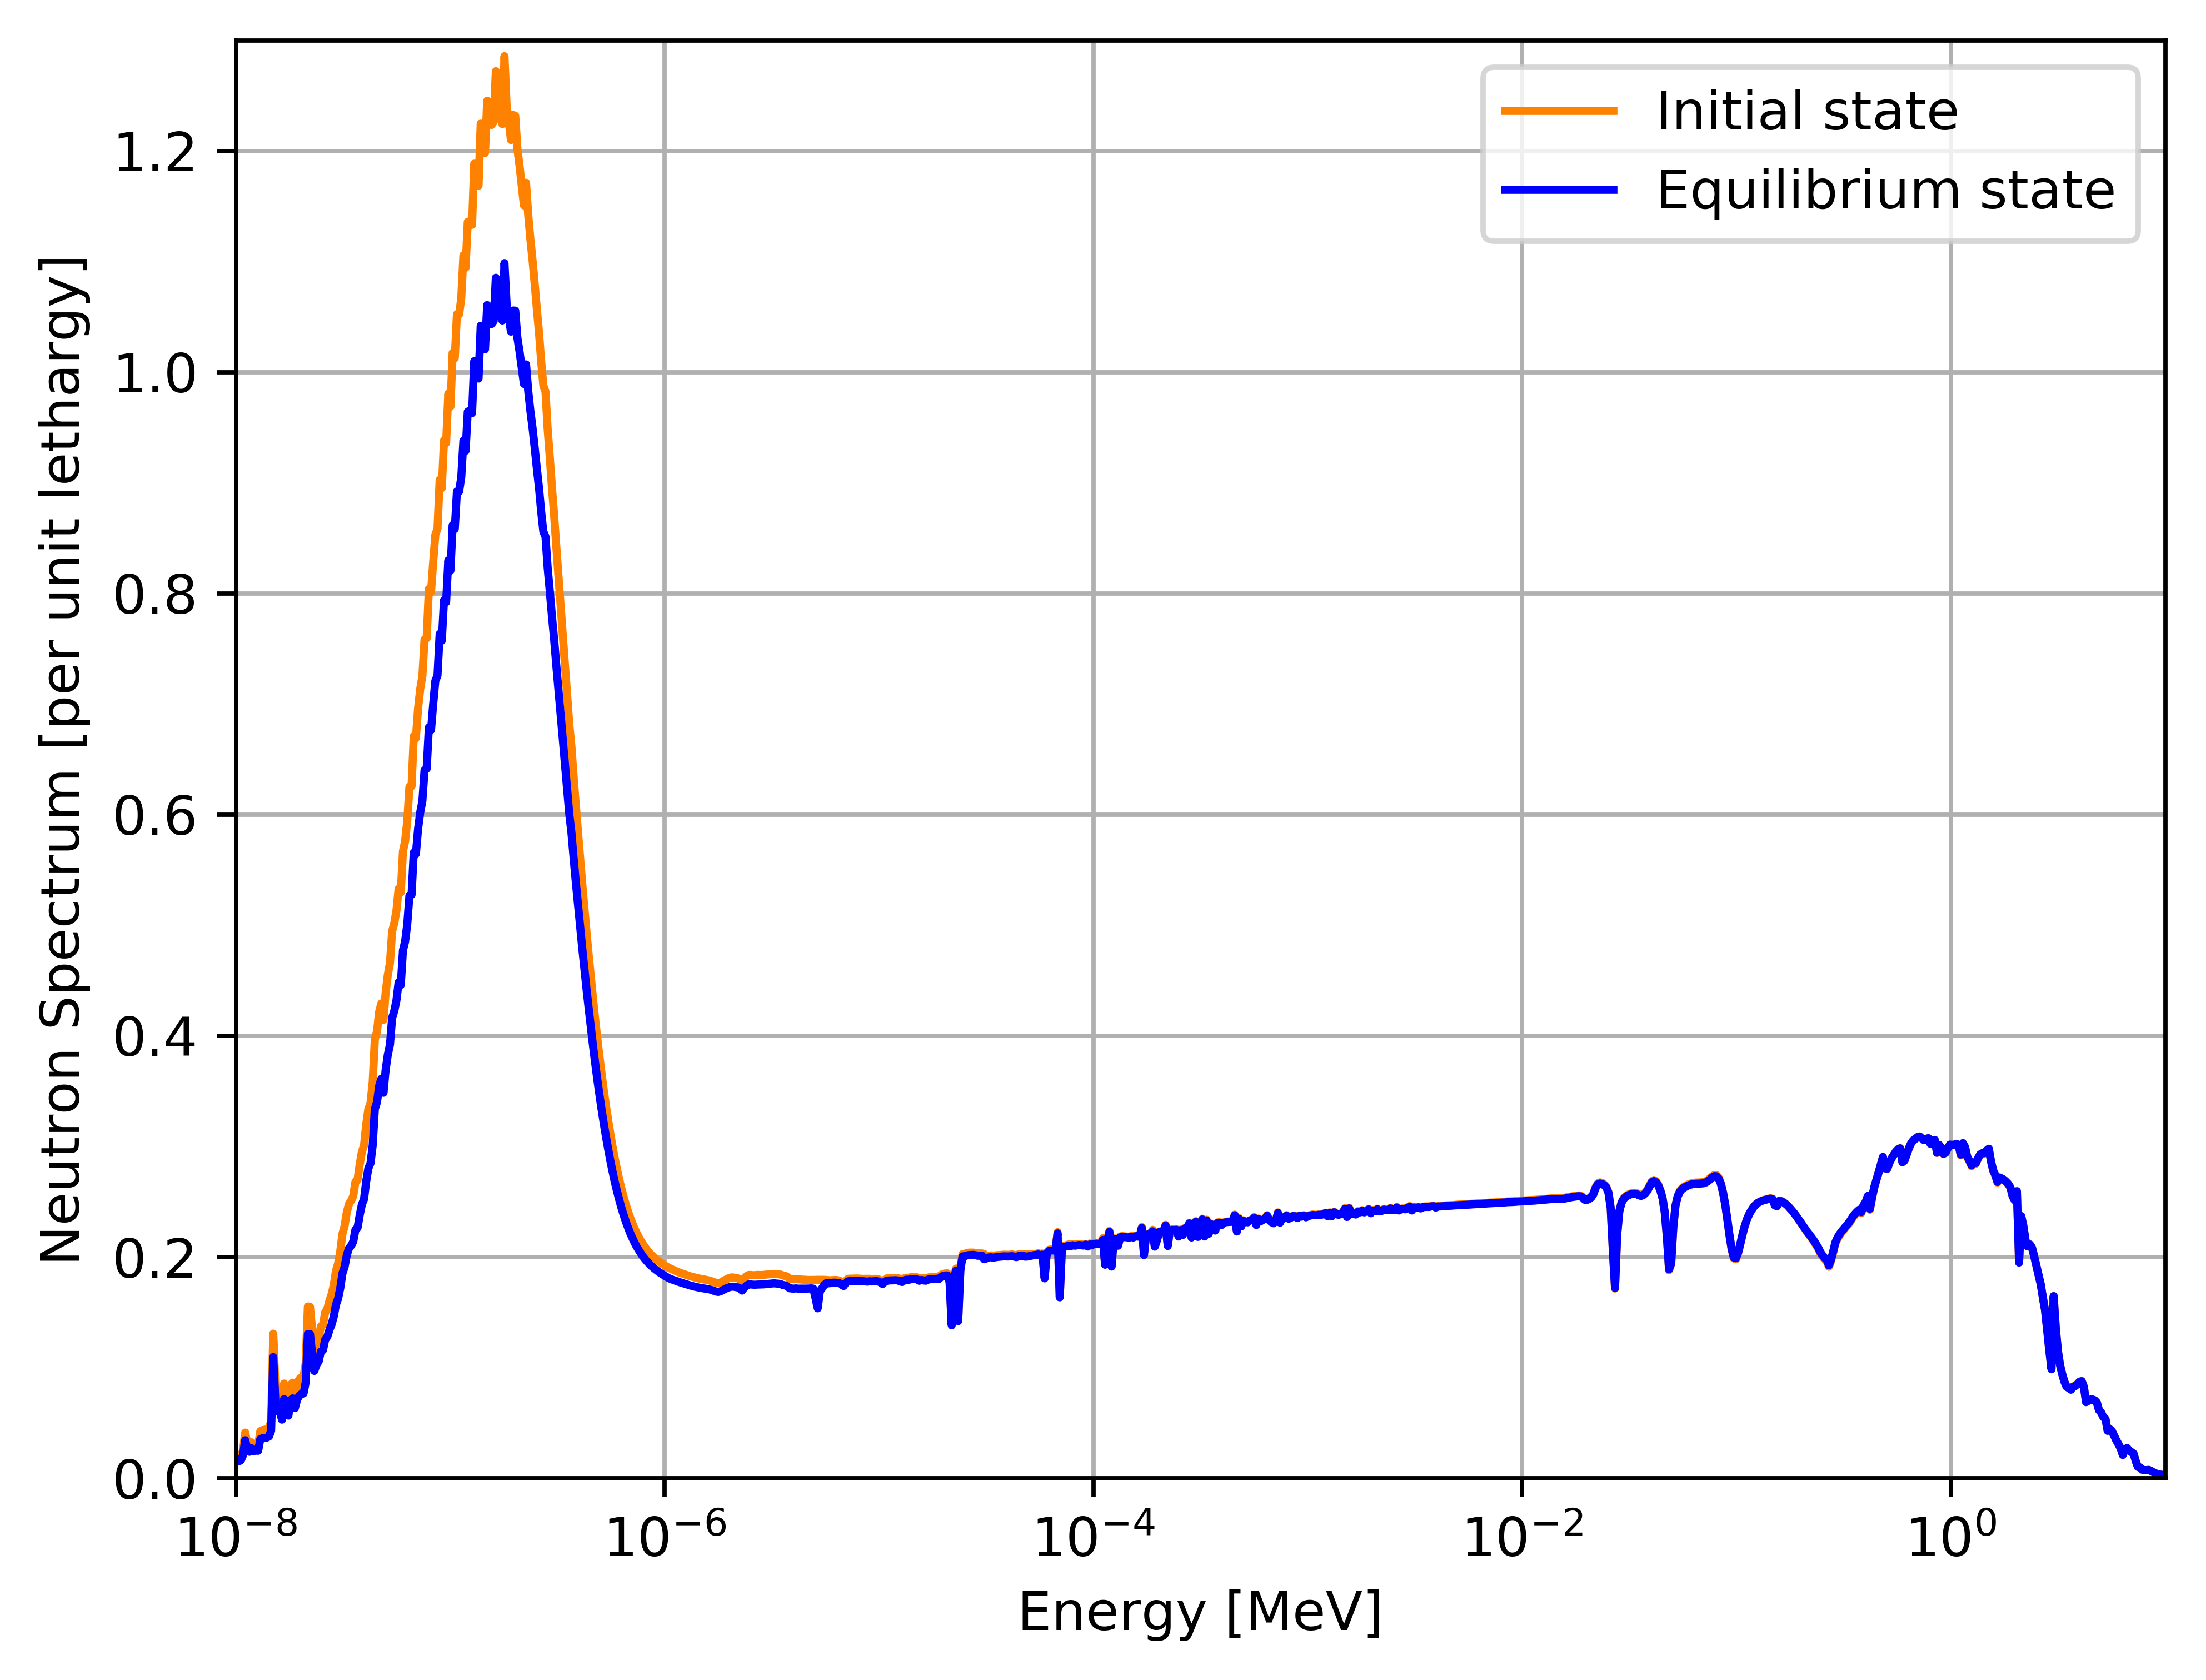
\includegraphics[width=\textwidth]{spectrum.png} \caption{The neutron flux energy 
  spectrum is normalized by unit lethargy and the area under the curve is normalized to 1 for initial and equilibrium fuel salt 
  composition.}
  \label{fig:spectrum}
\end{figure}

\begin{figure}[ht!] % replace 't' with 'b' to force it to 
  \centering
  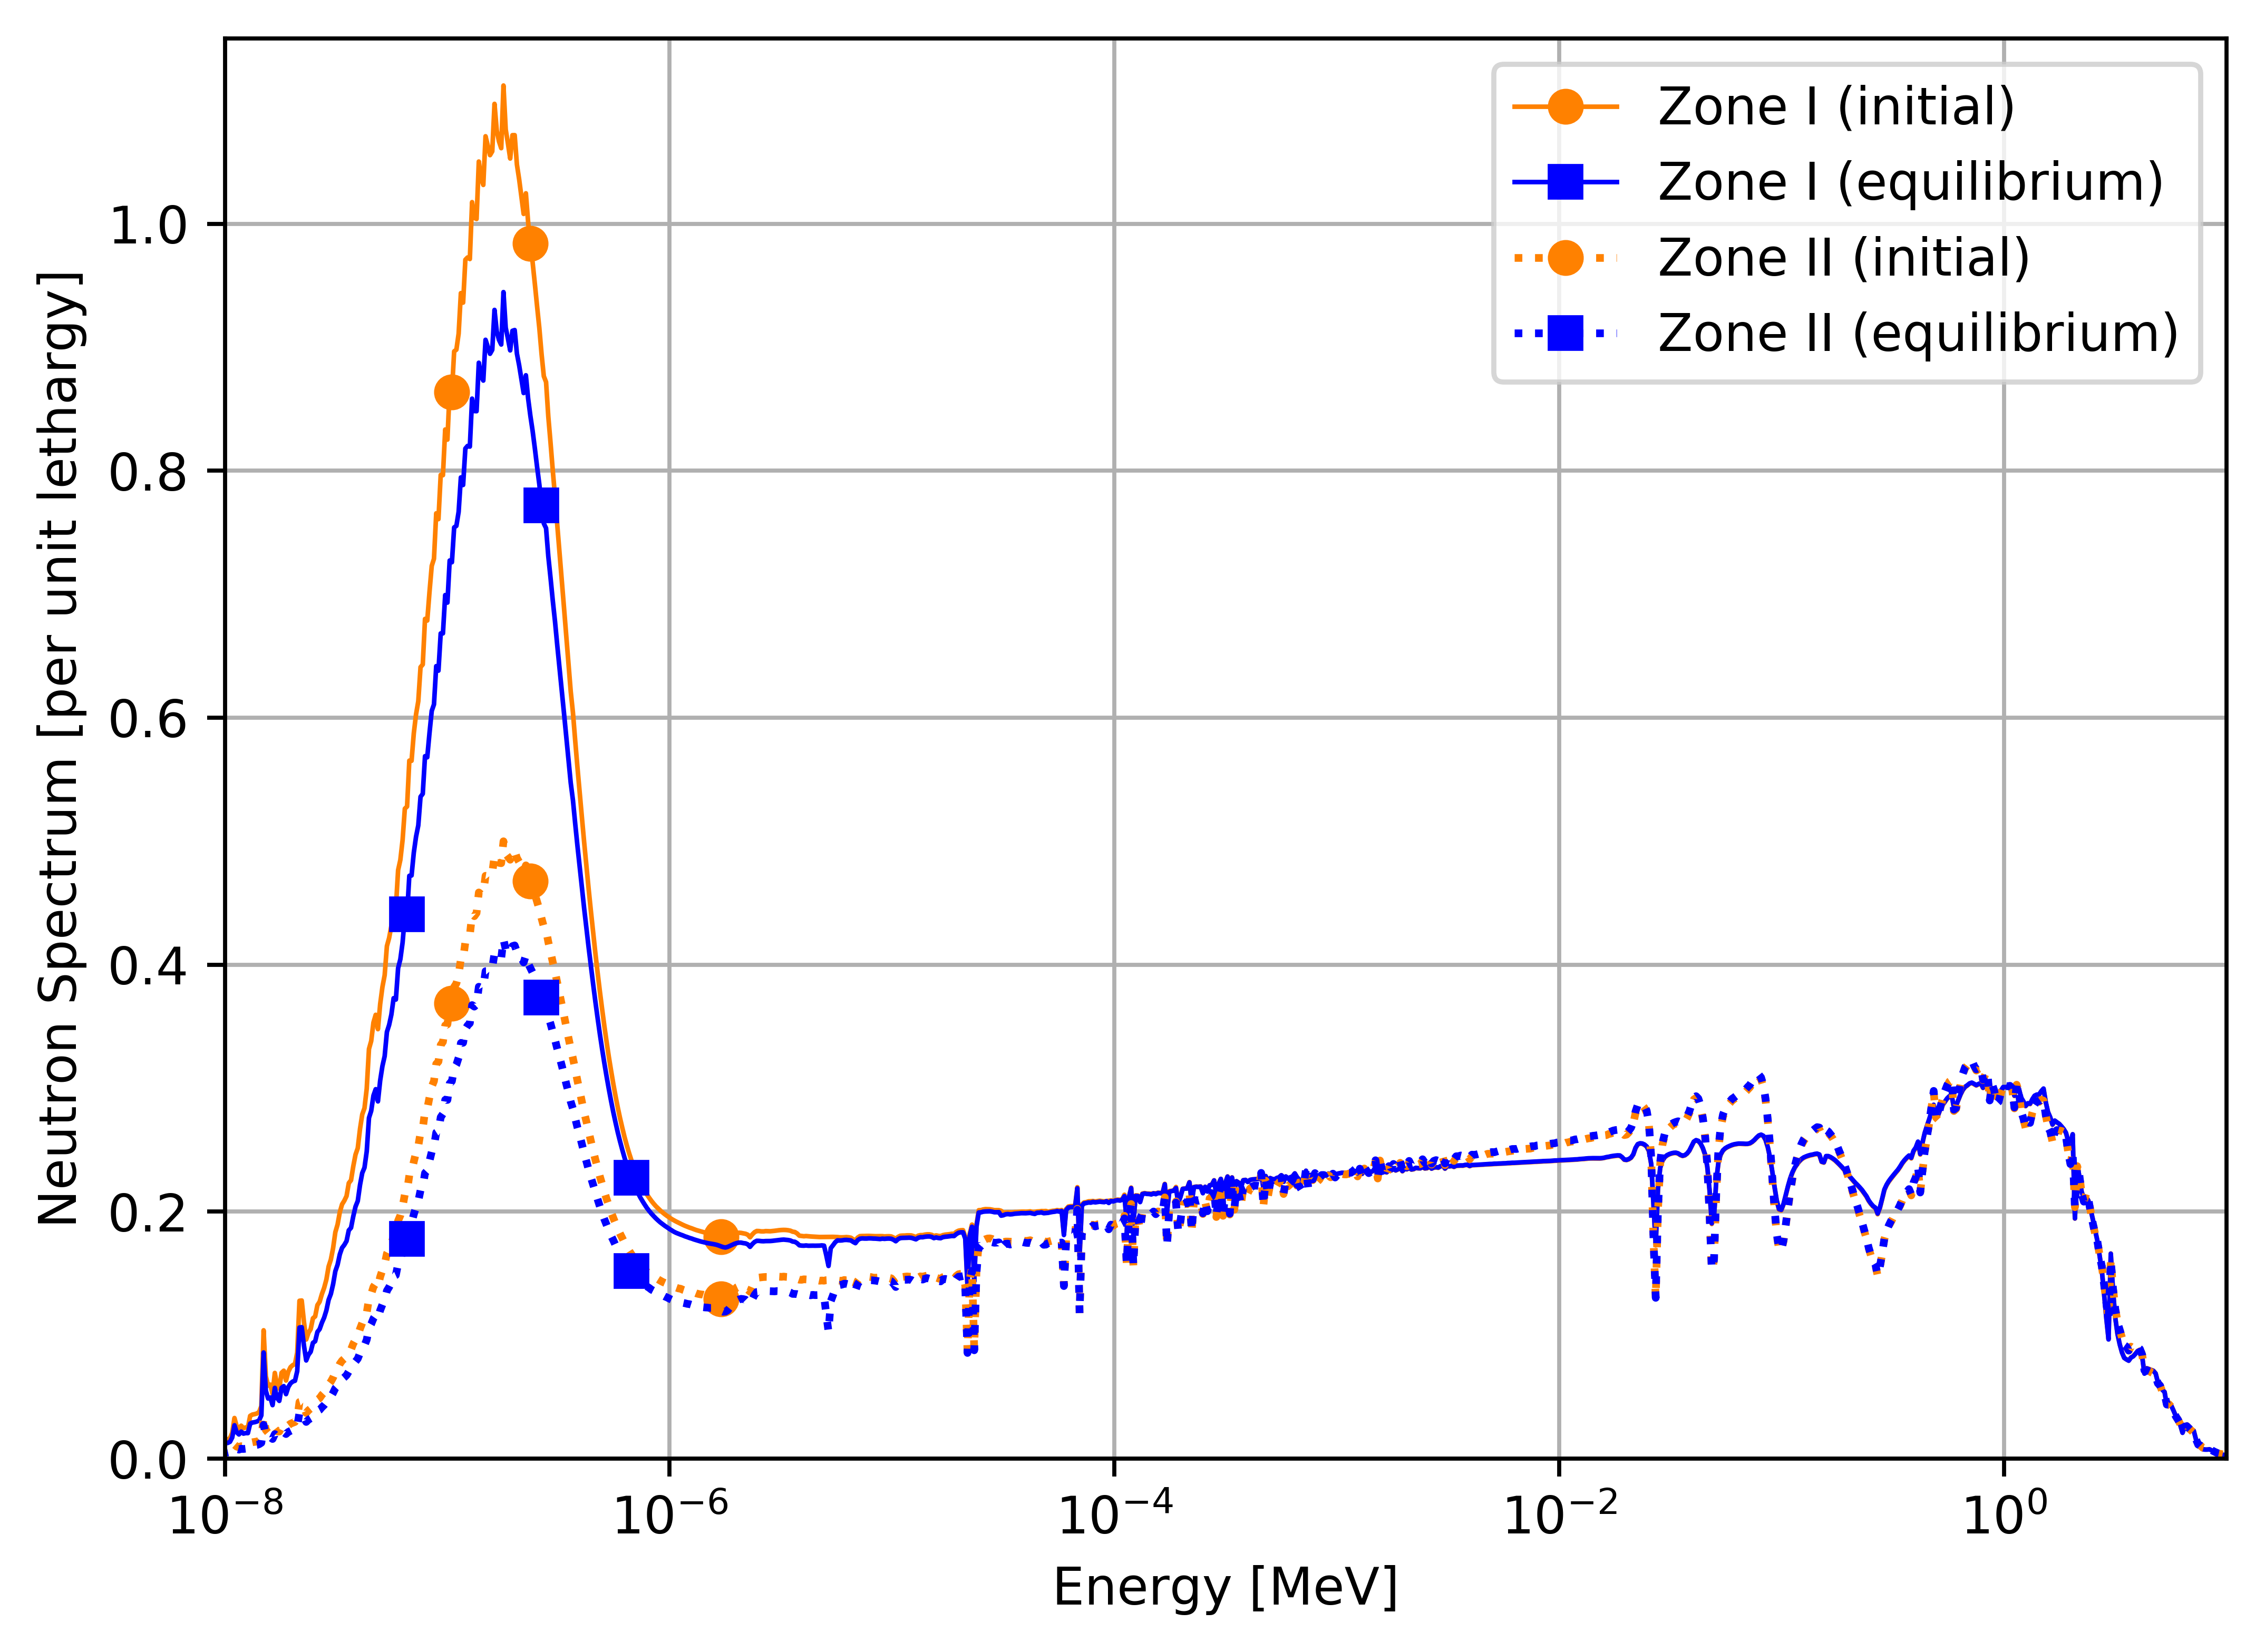
\includegraphics[width=\textwidth]{spectrum_zones.png} 
  \caption{The neutron flux energy spectrum in different core regions is normalized by 
unit lethargy and the area under the curve is normalized to 1 for the initial and equilibrium fuel salt composition.}
  \label{fig:spectrum_zones}
\end{figure}

\subsection{Neutron flux}
Figure~\ref{fig:radial_flux} shows the radial distribution of fast and thermal 
neutron flux for the both initial and equilibrium composition. 
\begin{figure}[ht!] % replace 't' with 'b' to force it to \centering
  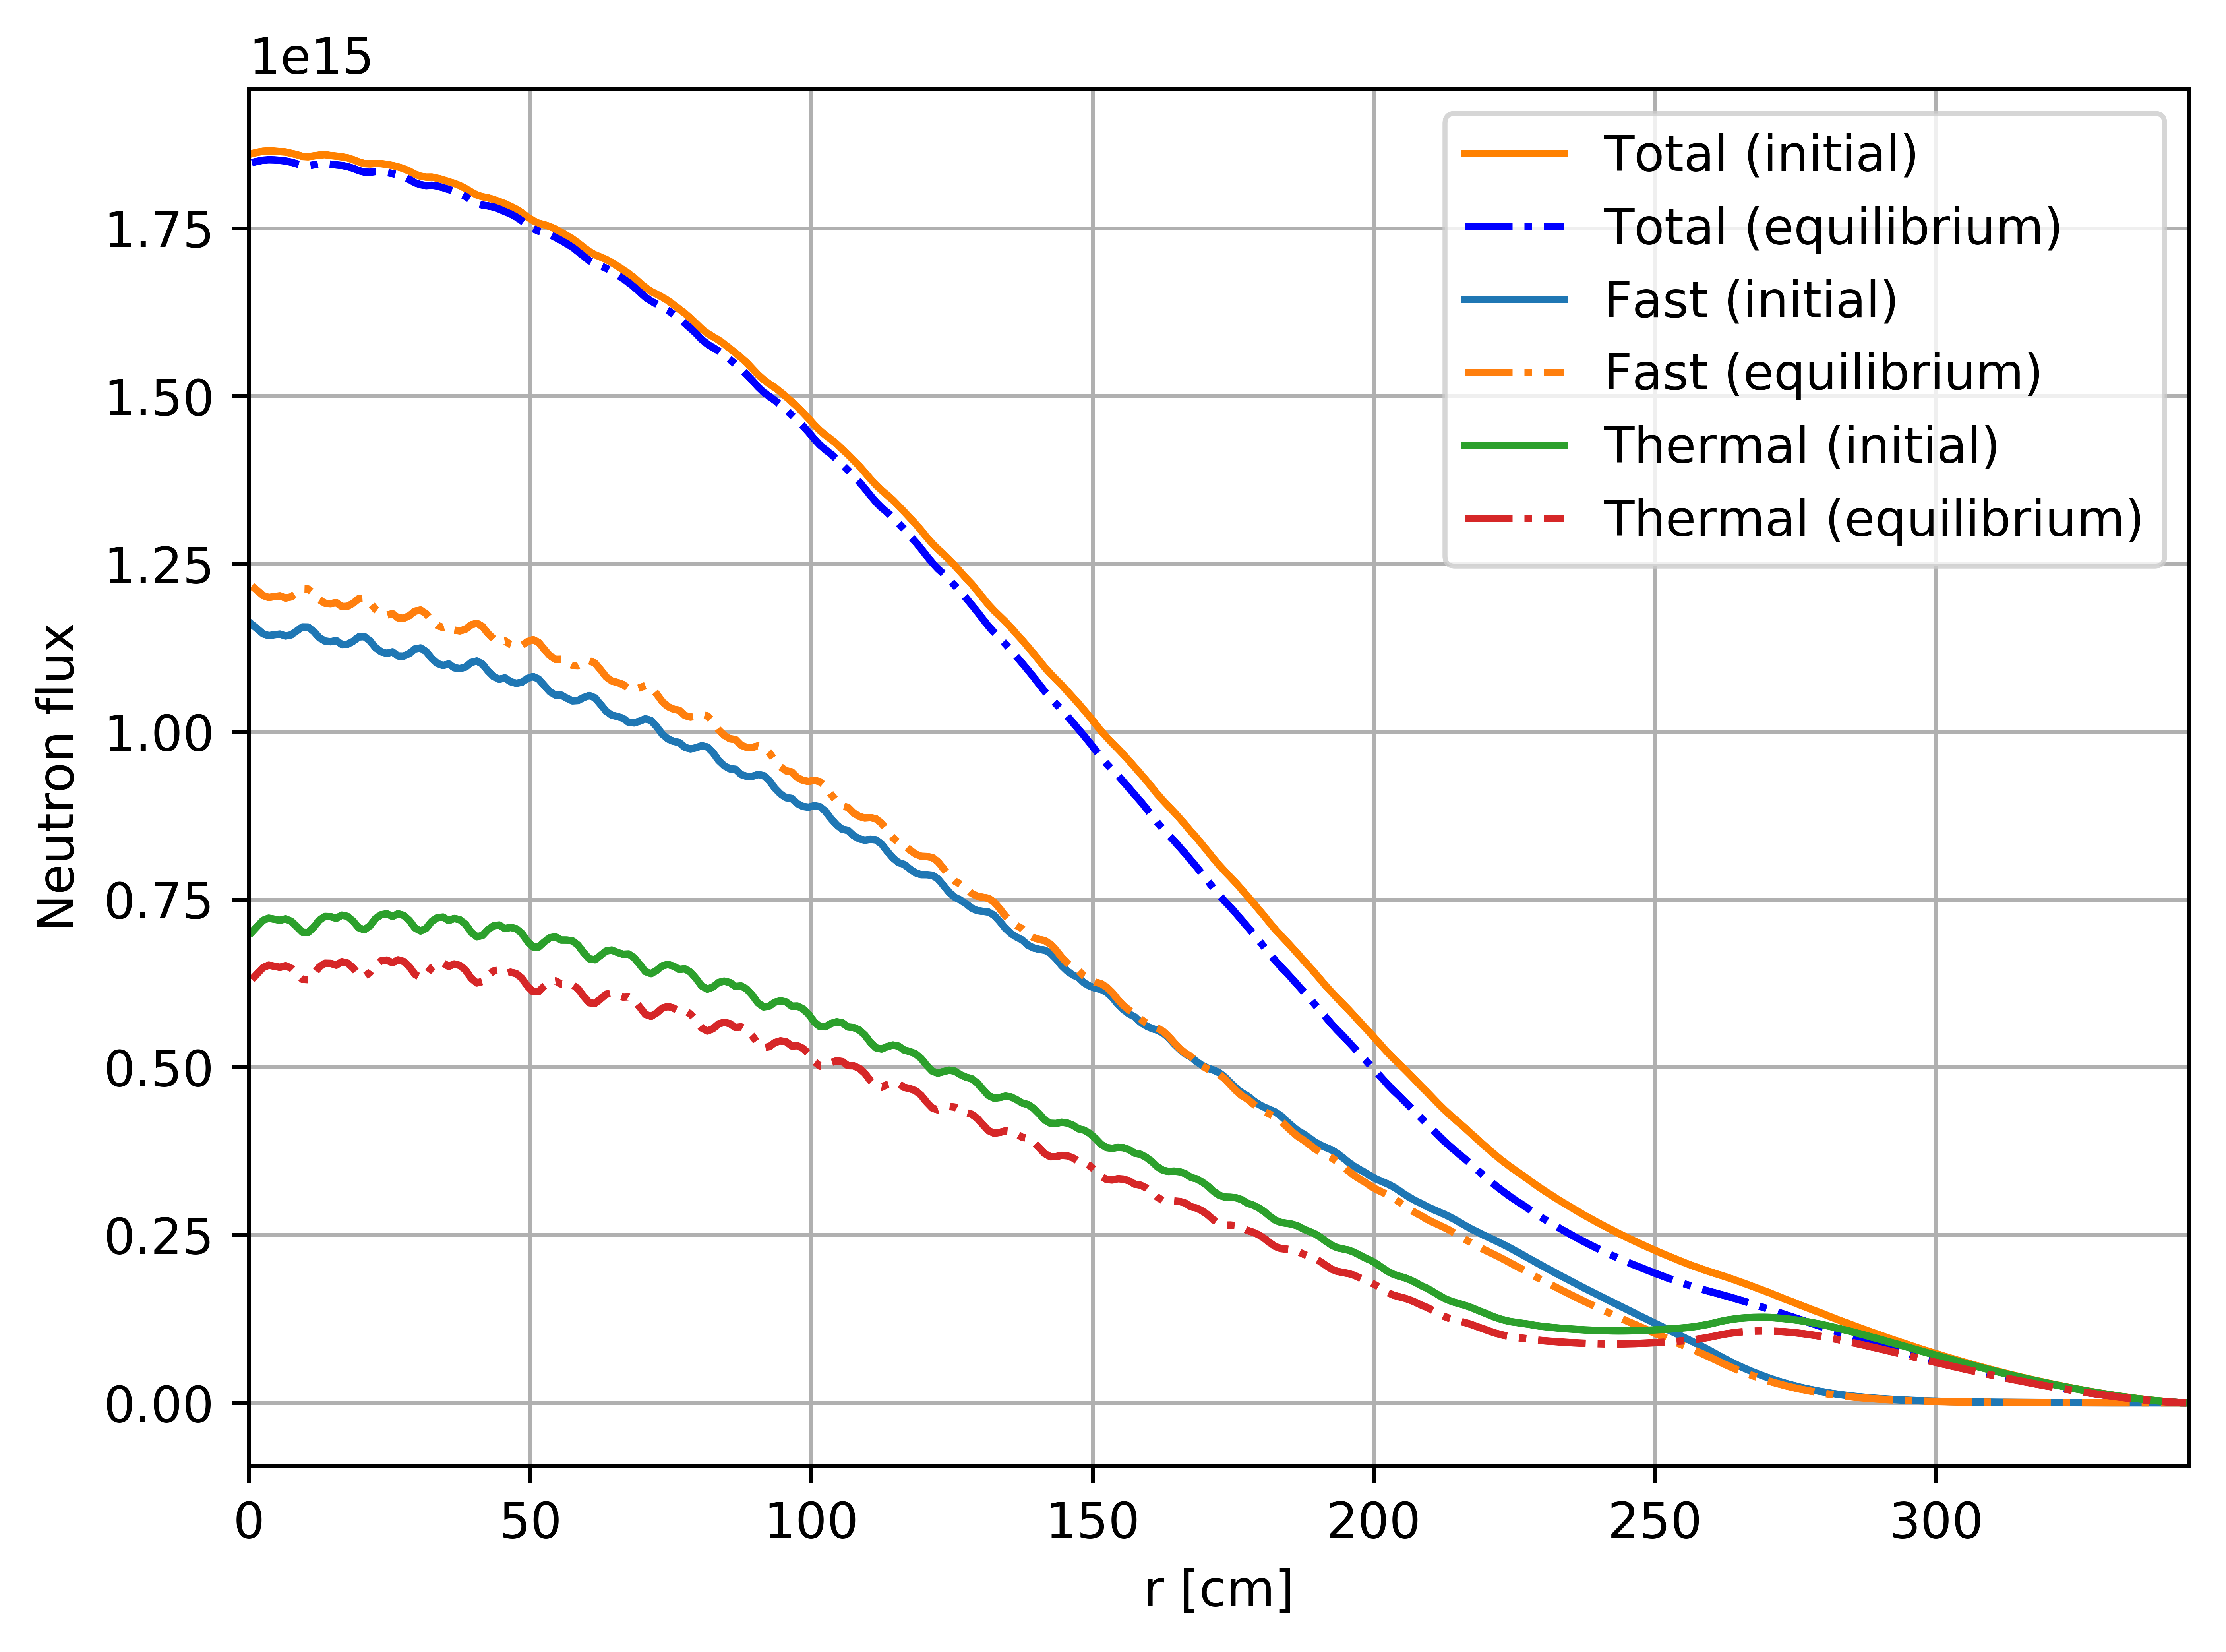
\includegraphics[width=\textwidth]{radial_flux.png} \caption{Radial neutron 
  flux distribution for initial and equilibrium fuel salt composition.}
  \label{fig:radial_flux}
\end{figure}

\subsection{Power and breeding distribution}
Table~\ref{tab:powgen_fraction} shows the power fraction in each zone for 
initial and equilibrium fuel compositions. Figure~\ref{fig:pow_den} reflects the 
normalized power distribution of the \gls{MSBR} quarter core for equilibrium fuel
 salt composition. For both the initial and equilibrium compositions, fission 
primarily occurs in the center of the core, namely zone I. The spectral shift 
during reactor operation results in slightly different power fractions at startup and 
equilibrium, but most of the power is still generated in zone I at equilibrium 
(table~\ref{tab:powgen_fraction}). 
%%%%%%%%%%%%%%%%%%%%%%%%%%%%%%%%%%%%%%%%
\begin{table}[ht!]
  \caption{Power generation fraction in each zone for initial and equilibrium 
  state.}
\begin{tabularx}{\textwidth}{ m | s | s } \hline
Core region      & Initial      & Equilibrium   \\   \hline
Zone I           & 97.91\%      & 98.12\%   \\
Zone II          & 2.09\%       & 1.88\%   \\ \hline
\end{tabularx}
  \label{tab:powgen_fraction}
\end{table}
%%%%%%%%%%%%%%%%%%%%%%%%%%%%%%%%%%%%%%%%%%%%%%%%%%%%%%%%%%%%%%%%%%%%%%%%%%%%%%%%
Figure~\ref{fig:breeding_den} shows the neutron capture reaction rate 
\begin{figure}[ht!] % replace 't' with 'b' to force it to \centering
  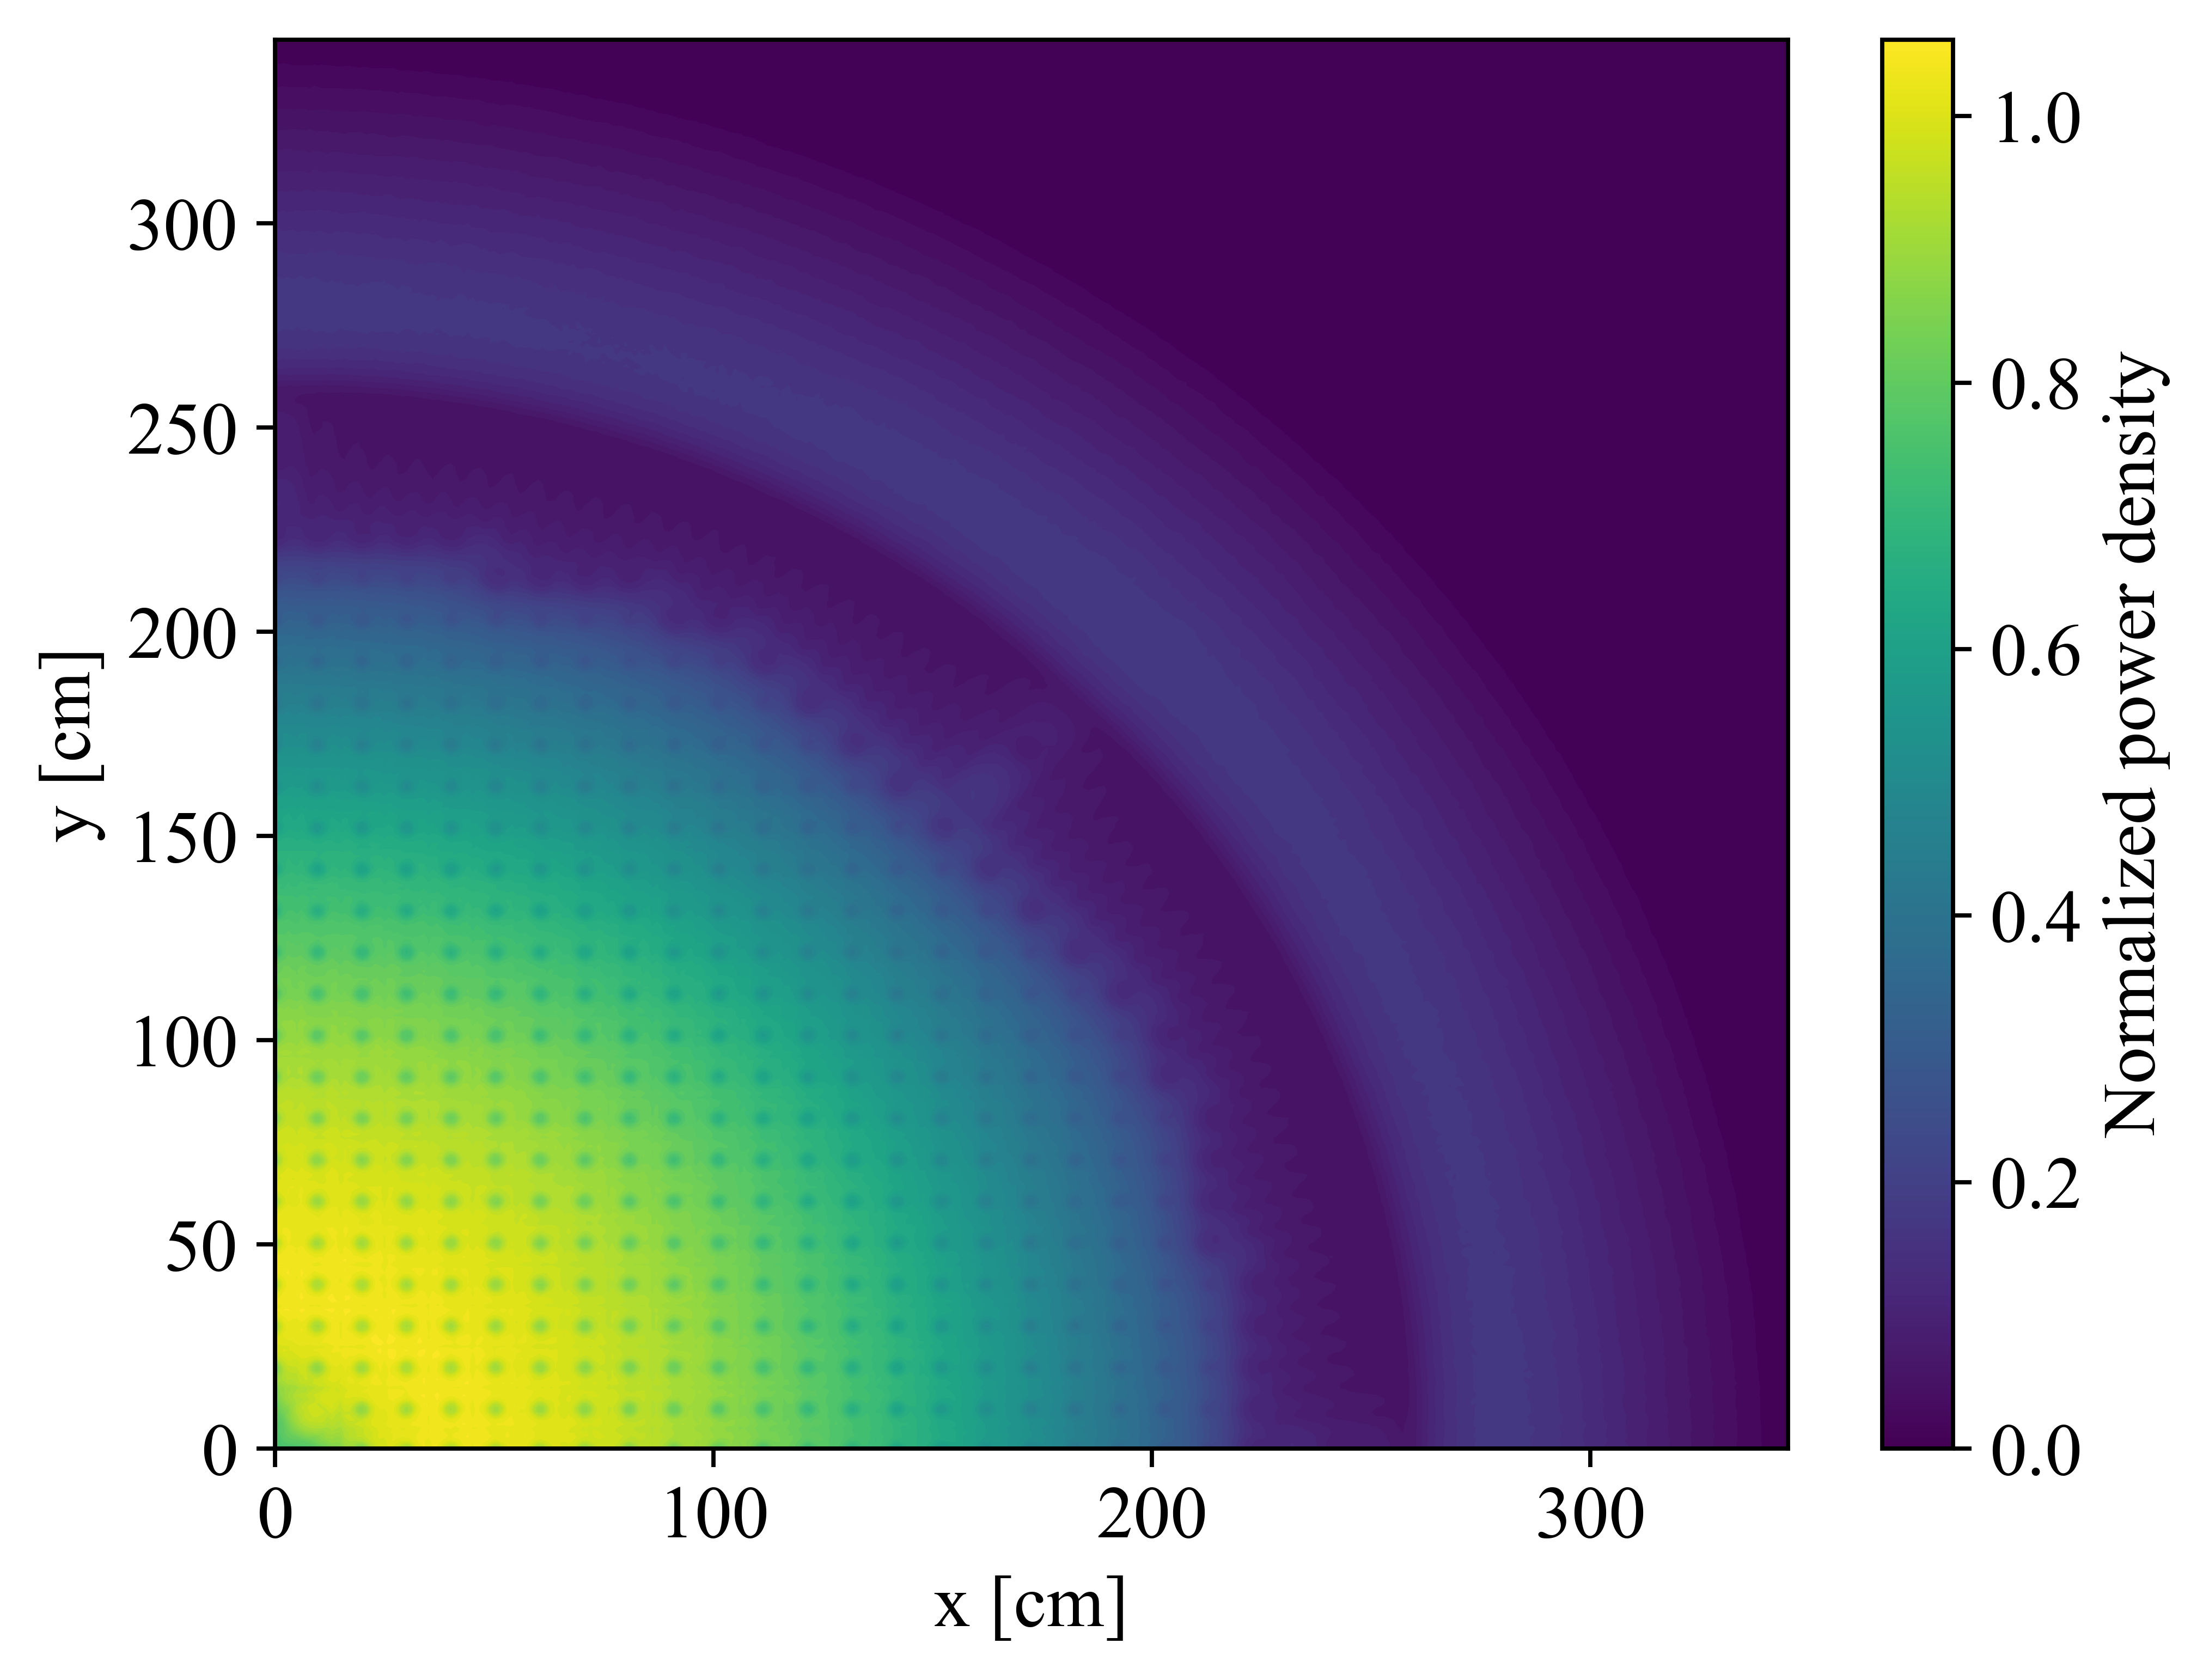
\includegraphics[width=\textwidth]{power_distribution_eq.png} 
  \caption{Normalized power density for equilibrium fuel salt 
  composition.}
  \label{fig:pow_den}
\end{figure}
\begin{figure}[ht!] % replace 't' with 'b' to force it to \centering
  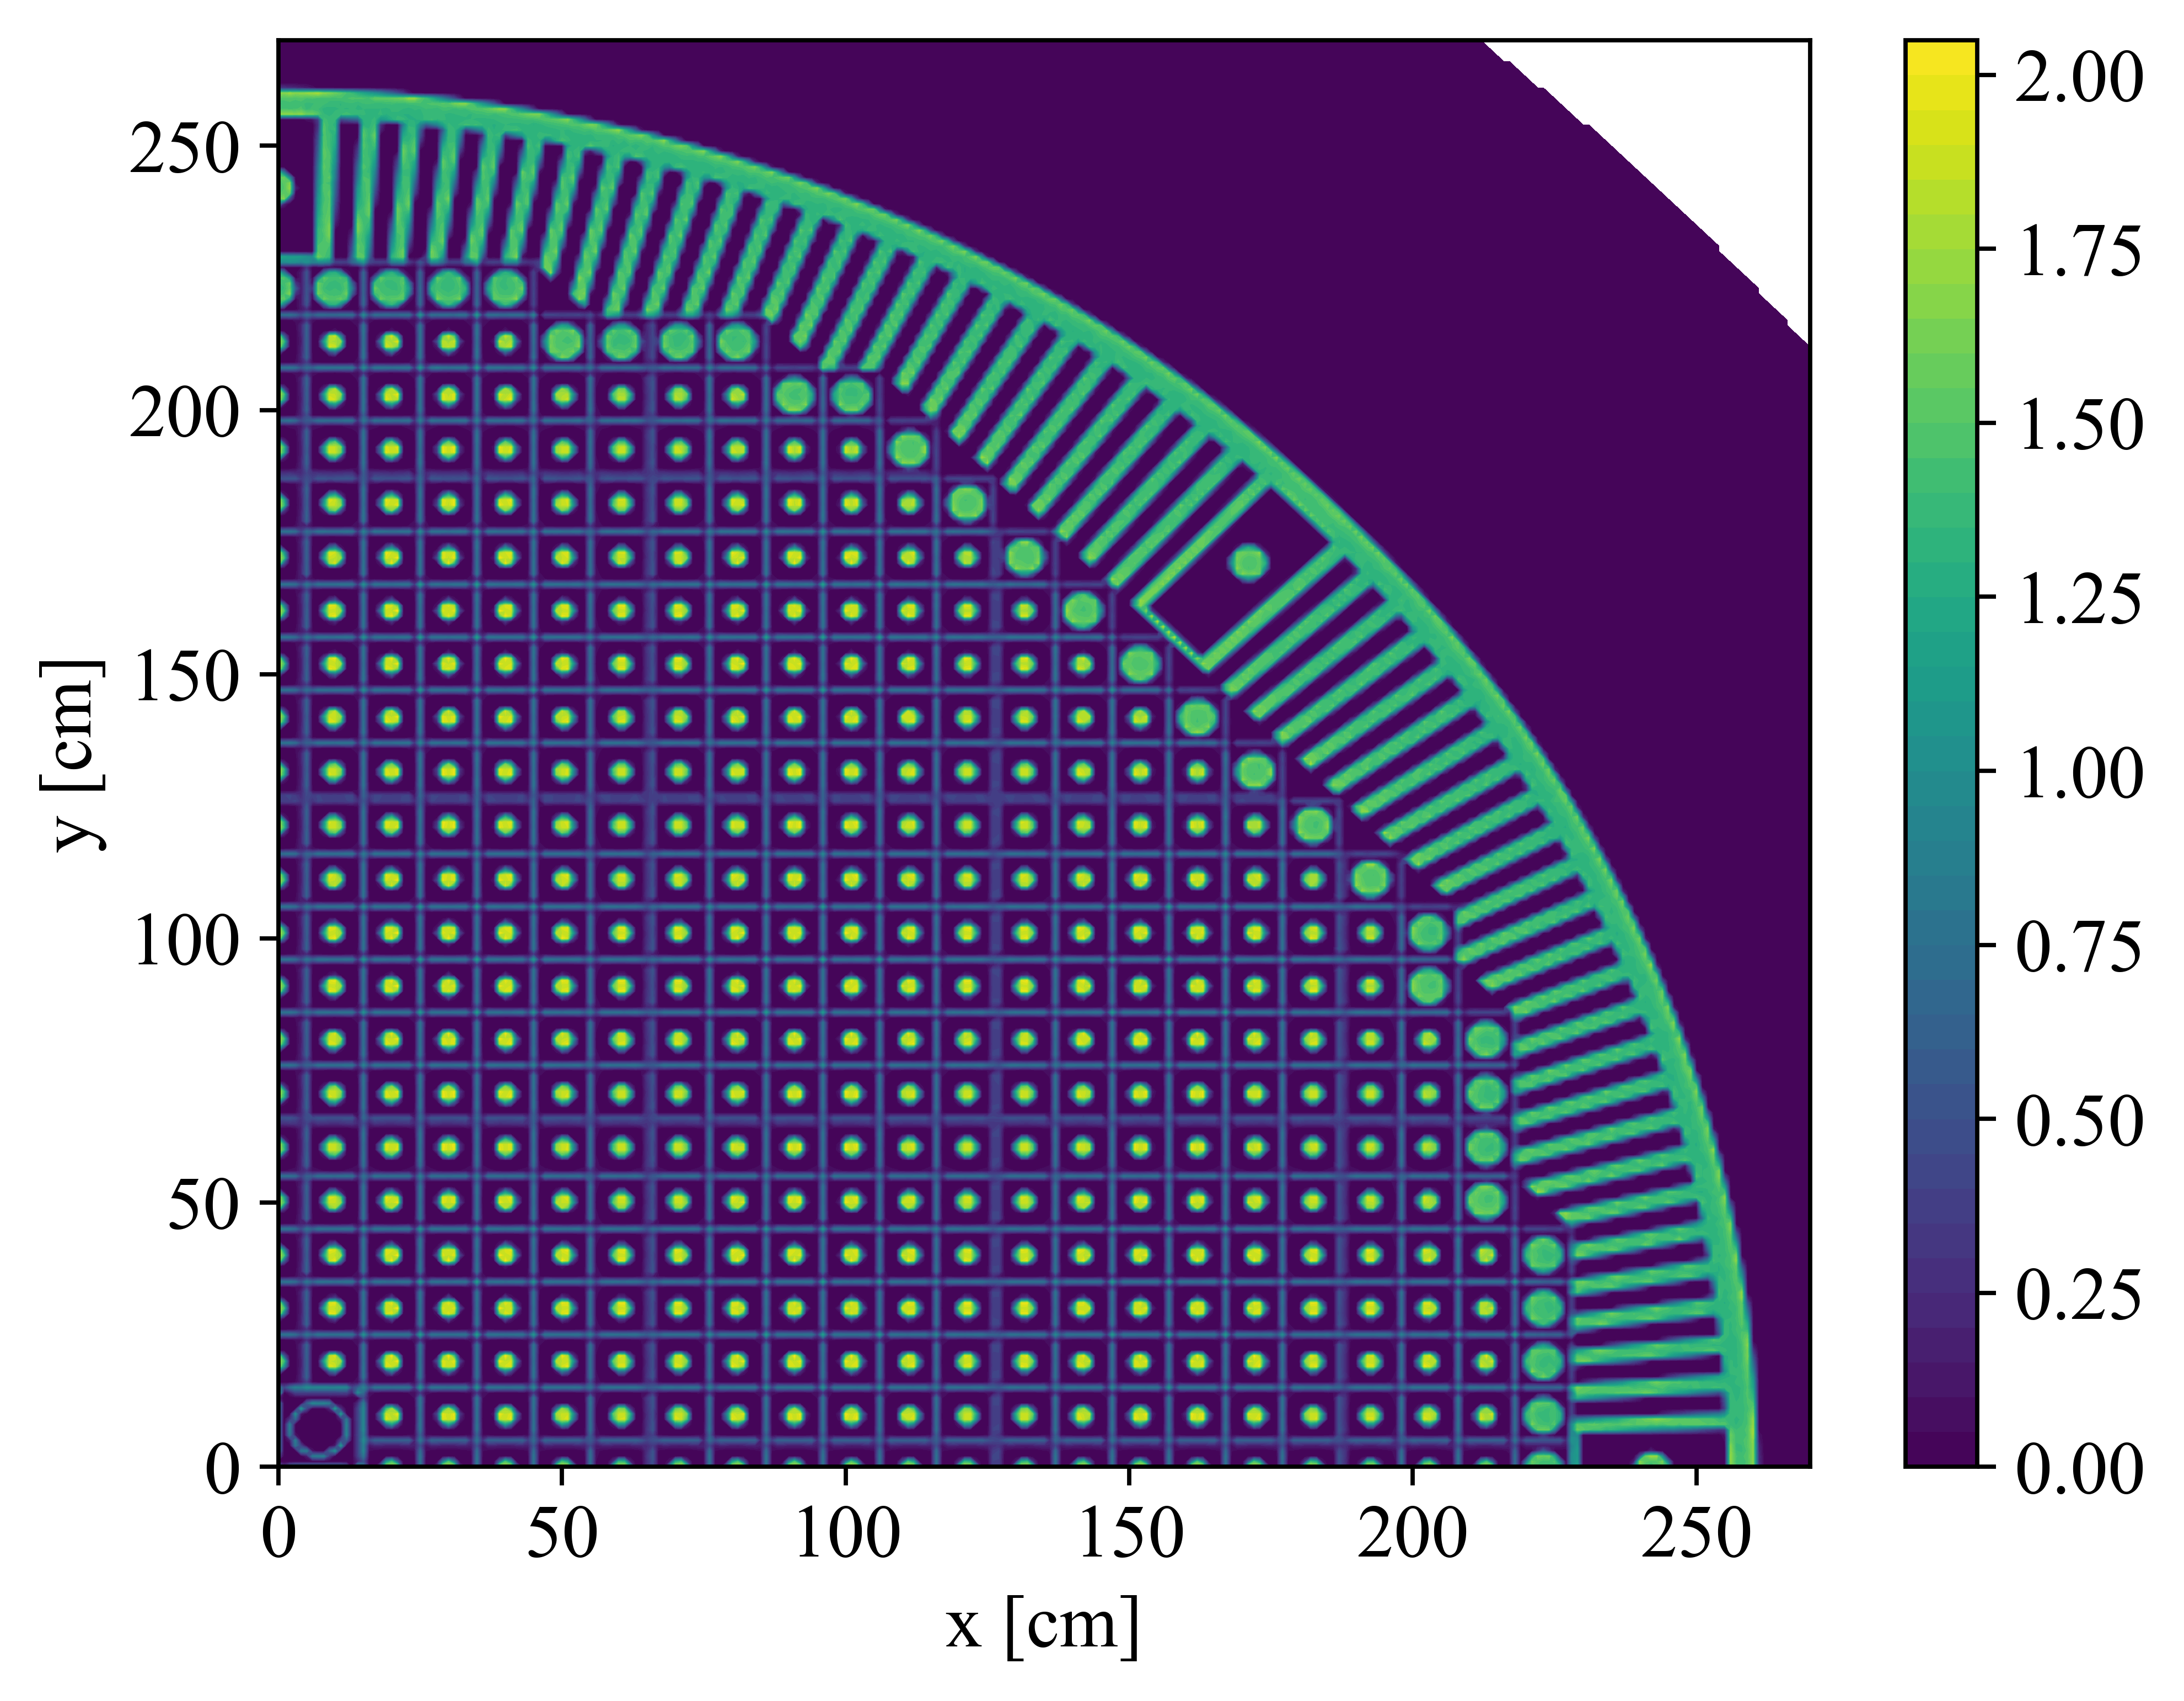
\includegraphics[width=\textwidth]{breeding_distribution_eq.png} 
  \caption{$^{232}$Th neutron capture reaction rate normalized by total flux 
  for equilibrium fuel salt composition.}
  \label{fig:breeding_den}
\end{figure}
\subsection{Temperature coefficient of reactivity}
Table~\ref{tab:tcoef} summarizes temperature effects on reactivity calculated 
in this work for both initial and equilibrium fuel compositions, compared 
with the original \gls{ORNL} report data \cite{robertson_conceptual_1971}. 
By propagating the $k_{eff}$  statistical error provided by SERPENT2, 
uncertainty for each temperature coefficient was obtained and appears in 
Table~\ref{tab:tcoef}. Other sources of uncertainty are neglected, such as cross section 
measurement error and approximations inherent in the equations of state 
providing both the salt and graphite density dependence on temperature.
 The main physical principle underlying the reactor 
temperature feedback is an expansion of heated material. When the fuel 
salt temperature increases, the density of the salt decreases, but at the same 
time, the total volume of fuel salt in the core remains constant because it is 
bounded by the graphite. When the graphite temperature increases, the density 
of graphite decreases, creating additional space for fuel salt. To determine 
the temperature coefficients, the cross section temperatures for the fuel and 
moderator were changed from 900K to 1000K. Three different cases were considered:
\begin{enumerate}
  \item Temperature of fuel salt rising from 900K to 1000K.
  \item Temperature of graphite rising from 900K to 1000K.
  \item Whole reactor temperature rising from 900K to 1000K.
\end{enumerate}
%%%%%%%%%%%%%%%%%%%%%%%%%%%%%%%%%%%%%%%%
\begin{table}[ht!]
  \caption{Temperature coefficients of reactivity for initial and equilibrium 
  state.}
\begin{tabularx}{\textwidth}{ X | r | r | r } \hline
Reactivity coefficient               & Initial         & Equilibrium     & Reference                                 \\ 
                                        & [pcm/k]         &  [pcm/k]        & (initial/equilibrium)\cite{li_optimization_2018} \tabularnewline  \hline
Doppler in fuel salt                    & $-4.70\pm0.159$ & $-5.30\pm0.186$ & 
\tabularnewline
Fuel salt density                       & $+1.19\pm0.155$ & $+2.93\pm0.186$ & 
\tabularnewline
Total fuel salt                         & $-3.67\pm0.157$ & $-2.62\pm0.189$ & 
\tabularnewline \hline
Doppler in graphite                     & $+2.00\pm0.158$ & $+0.85\pm0.188$ &          \tabularnewline
Total moderator (graphite)              & $+2.00\pm0.158$ & $+0.85\pm0.188$ & 
\tabularnewline \hline
Total core                              & $-1.45\pm0.159$ & $-2.04\pm0.186$ & $-2.0/-1.8$  \tabularnewline \hline
\end{tabularx}
  \label{tab:tcoef}
\end{table}
%%%%%%%%%%%%%%%%%%%%%%%%%%%%%%%%%%%%%%%%%%%%%%%%%%%%%%%%%%%%%%%%%%%%%%%%%%%%%%%%
In the first case, changes in the fuel temperature only impact fuel density. In 
this case, the geometry is unchanged because the fuel is a liquid. However, 
when the moderator heats up, both the density and the geometry change due to 
thermal expansion of the solid graphite blocks and reflector. Accordingly, the 
new graphite density was calculated using a linear temperature expansion 
coefficient of 1.3$\times10^{-6}$K$^{-1}$ \cite{robertson_conceptual_1971}. A new 
geometry input for SERPENT2, which takes into account displacement of graphite 
surfaces, was created based on this information. For calculation of 
displacement, it was assumed that the interface between the graphite reflector and vessel did not move,
 and that the vessel temperature did not change. This is the most reasonable assumption for
 the short-term reactivity effects because inlet salt is cooling graphite reflector and 
inner surface of the vessel.

The fuel temperature coefficient (FTC) is negative for both initial and 
equilibrium fuel compositions due to thermal Doppler broadening of the resonance 
capture cross sections in the thorium. A small positive effect of fuel density on 
reactivity increases from $+1.21$ pcm/K at reactor startup to $+1.66$ pcm/K for 
equilibrium fuel composition which has a negative effect on FTC magnitude during the 
reactor operation. This is in good agreement with earlier 
research \cite{robertson_conceptual_1971,park_whole_2015}. The moderator 
temperature coefficient (MTC) is positive for the startup composition and decreases 
during reactor operation because of spectrum hardening with fuel depletion. 
Finally, the total temperature coefficient of reactivity is negative for both 
cases, but decreases during reactor operation due to spectral shift. In 
summary, even after 20 years of operation the total temperature coefficient of 
reactivity is relatively large and negative during reactor operation (comparing 
with conventional PWR which has temperature coefficient about -1.71 pcm/$^\circ$F 
$\approx$ -3.08 pcm/K \cite{forget_integral_2018}), despite positive MTC, and 
affords excellent reactor stability and control.

\subsection{Six Factor Analysis}
The effective multiplication factor can be expressed using the following formula:
\begin{align*}
k_{eff} = k_{inf} P_f  P_t = \eta \epsilon p f P_f P_t
\end{align*}

Table~\ref{tab:six_factor} summarizes the six factors for both initial and 
equilibrium fuel salt composition. Using SERPENT2 and SaltProc, these factors and their statistical uncertainties
 have been calculated for both initial and equilibrium fuel salt composition (see 
Table~\ref{tab:msbr_tab}). The fast and thermal non-leakage probabilities 
remain constant despite the evolving neutron spectrum during operation. In 
contrast, the neutron reproduction factor ($\eta$), resonance escape 
probability ($p$), and fast fission factor ($\epsilon$) are considerably different between startup and 
equilibrium. As indicated in Figure~\ref{fig:spectrum}, the neutron spectrum is 
softer at the beginning of reactor life. Neutron spectrum hardening causes the fast 
fission factor to increase through the core lifetime. The opposite is true for the 
resonance escape probability. Finally, the neutron reproduction factor 
decreases during reactor operation due to accumulation of fissile plutonium 
isotopes.
%%%%%%%%%%%%%%%%%%%%%%%%%%%%%%%%%%%%%%%%
\begin{table}[hb!]
  \caption{Six factors for the full-core \gls{MSBR} model for initial and 
  equilibrium fuel composition.}
\begin{tabularx}{\textwidth}{ b | s | s } \hline
Factor  & Initial      & Equilibrium   \\ \hline
Neutron reproduction factor ($\eta$)     & $1.3960\pm.000052$     & 
        $1.3778\pm.00005$ \\ Thermal utilization factor (f)           & 
        $0.9670\pm.000011$     & $0.9706\pm.00001$ \\
Resonance escape probability (p)         & $0.6044\pm.000039$     & 
        $0.5761\pm.00004$ \\
Fast fission factor ($\epsilon$)         & $1.3421\pm.000040$     & 
        $1.3609\pm.00004$ \\
Fast non-leakage probability (P$_f$)     & $0.9999\pm.000004$     & 
        $0.9999\pm.000004$ \\
Thermal non-leakage probability (P$_t$)  & $0.9894\pm.000005$     & 
        $0.9912\pm.00005$ \\ \hline
\end{tabularx}
  \label{tab:six_factor}
\end{table}
%%%%%%%%%%%%%%%%%%%%%%%%%%%%%%%%%%%%%%%%%%%%%%%%%%%%%%%%%%%%%%%%%%%%%%%%%%%%%%%%
\subsection{Thorium refill rate and U233 production}

\FloatBarrier
%\section{Discussion}
% This should explore the significance of the results of the work, not repeat
% them. A combined Results and Discussion section is often appropriate. Avoid
% extensive citations and discussion of published literature.
Short 2-3 paragraph discussion. This will emphasize:
\begin{itemize}
  \item Discuss reason of spectral shift (heavy \gls{FP} accumulation, Pu isotopes).
  \item Neutron spectral shift which causes safety parameters worsening.  
  \item Couple words about power profile.
\end{itemize}

%\FloatBarrier
\section{Discussion and conclusions}

\FloatBarrier
\section{Acknowledgments}

This research is part of the Blue Waters sustained-petascale computing project, 
which is supported by the National Science Foundation (awards OCI-0725070 and 
ACI-1238993) and the state of Illinois. Blue Waters is a joint effort of the 
University of Illinois at Urbana-Champaign and its National Center for 
Supercomputing Applications 

The authors contributed to this work as described below. Osama Ashraf
conceived and designed the simulations, wrote the paper, prepared figures 
and/or tables, performed the computation work, and reviewed drafts of the paper. Osama Ashraf
is supported by ...........................

Andrei Rykhlevskii conceived and designed the simulations, wrote the paper, prepared figures 
and/or tables, performed the computation work, contributed to the software 
product, and reviewed drafts of the paper. Andrei Rykhlevskii 
is supported by DOE ARPA-E MEITNER program award 1798-1576. 

Kathryn D. Huff directed and supervised the work, conceived and designed the simulations, contributed to the software product, and reviewed drafts of the paper.  Prof. Huff is supported by the Nuclear Regulatory Commission Faculty Development Program, the National Center for Supercomputing Applications, the NNSA Office of Defense Nuclear Nonproliferation R\&D through the Consortium for Verfication Technologies and the Consortium for Nonproliferation Enabling Capabilities,  the International Institute for Carbon Neutral Energy Research (WPI-I2CNER), 
sponsored by the Japanese Ministry of Education, Culture, Sports, Science and Technology, and DOE ARPA-E MEITNER program award 1798-1576. 


\FloatBarrier

\nocite{robertson_conceptual_1971} % placeholder until citations appear
\bibliography{2019-tmsr-serpent.bib}

\end{document}
